
\documentclass[12pt]{report}
\usepackage{textcomp}

\addtolength{\hoffset}{-2.25cm}
\addtolength{\textwidth}{4.5cm}
\addtolength{\voffset}{-2.5cm}
\addtolength{\textheight}{5cm}
\setlength{\parskip}{0pt}
\setlength{\parindent}{15pt}

\usepackage{graphicx}
\graphicspath{ {./images/} }

\usepackage{amsthm}
\usepackage{amsmath}
\usepackage{amssymb}

\usepackage[colorlinks = true, linkcolor = black, citecolor = black, final]{hyperref}

\usepackage{graphicx}
\usepackage{multicol}
\usepackage{marvosym}
\usepackage{wasysym}

\usepackage{outlines}
\usepackage[utf8]{inputenc}
\usepackage[english]{babel}

\usepackage{enumitem,amssymb}

\newcommand{\pr}[1]{\left(#1\right)}

\usepackage{pgfplots}
\pgfplotsset{compat=1.16}
\usepackage{circuitikz}
\usepackage{tikz}
\usetikzlibrary{patterns}
\usetikzlibrary{arrows.meta}

\usepackage{mdframed}
\usepackage{pbox}
\usepackage{array}
\usepackage{makecell}
\usepackage{booktabs}
\setlength{\heavyrulewidth}{1pt}
\setlength{\abovetopsep}{4pt}


\setlength{\parindent}{0in}

\pagestyle{plain}

\definecolor{codegreen}{rgb}{0,0.6,0}
\definecolor{codegray}{rgb}{0.5,0.5,0.5}
\definecolor{codepurple}{rgb}{0.58,0,0.82}
\definecolor{backcolour}{rgb}{0.95,0.95,0.92}
\definecolor{backcolour2}{rgb}{0.44,0.63,0.99}

\definecolor{dkgreen}{rgb}{0,0.6,0}
\definecolor{gray}{rgb}{0.5,0.5,0.5}
\definecolor{mauve}{rgb}{0.58,0,0.82}

\usepackage{listings}
\lstset{
    language=Verilog,
    breakatwhitespace=false,         
    breaklines=true,                 
    captionpos=b,                    
    keepspaces=true,                 
    numbers=left,                    
    numbersep=5pt,                  
    showspaces=false,                
    showstringspaces=false,
    showtabs=false       
    columns=flexible,
    basicstyle={\small\ttfamily},
    numberstyle=\tiny\color{gray},
    keywordstyle=\color{blue},
    commentstyle=\color{dkgreen},
     % stringstyle=\color{mauve},
    stringstyle=\color{orange},
    backgroundcolor=\color{backcolour},
    tabsize=4  
}

\lstnewenvironment{CPP}
  {\lstset{language=C,basicstyle=\ttfamily\small,frame=none}}
  {}

%%%%%%%%%%%%%%%% These commands are taken from Professor Ashmanskas!
\newcommand{\ohm}{\Omega}
\newcommand{\kohm}{{\rm k}\Omega}
\newcommand{\Mohm}{{\rm M}\Omega}
\newcommand{\dif}{{\rm d}}
\newcommand{\kgmps}{{\rm kg\cdot m/s}}
\newcommand{\degC}{{}^\circ{\rm C}}
\newcommand{\degF}{{}^\circ{\rm F}}
\newcommand{\K}{{\rm K}}
\newcommand{\liter}{{\rm L}}
\newcommand{\mL}{{\rm mL}}
\newcommand{\atm}{{\rm atm}}
\newcommand{\mol}{{\rm mol}}
\newcommand{\Cal}{{\rm Cal}}
\newcommand{\W}{{\rm W}}
\newcommand{\kW}{{\rm kW}}
\newcommand{\dB}{{\rm dB}}
\newcommand{\amu}{{\rm u}}
\newcommand{\Pa}{{\rm Pa}}
\newcommand{\J}{{\rm J}}
\newcommand{\N}{{\rm N}}
\newcommand{\pC}{{\rm pC}}
\newcommand{\C}{{\rm C}}
\newcommand{\T}{{\rm T}}
\newcommand{\eV}{{\rm eV}}
\newcommand{\V}{{\rm V}}
\newcommand{\mV}{{\rm mV}}
\newcommand{\Vpp}{{ V}_{ pp}}
\newcommand{\mVpp}{{\rm mV}_{\rm pp}}
\newcommand{\Vac}{{\rm V}_{\rm AC}}
\newcommand{\Vdc}{{\rm V}_{\rm DC}}
\newcommand{\Vbold}{{\bf V}}
\newcommand{\Ibold}{{\bf I}}
\newcommand{\Zbold}{{\bf Z}}
\newcommand{\kV}{{\rm kV}}
\newcommand{\emf}{{\cal E}}
\newcommand{\A}{{\rm A}}
\newcommand{\mA}{{\rm mA}}
\newcommand{\uA}{{\rm \mu A}}
\newcommand{\nA}{{\rm nA}}
\newcommand{\F}{{\rm F}}
\newcommand{\uF}{\mu{\rm F}}
\newcommand{\nF}{{\rm nF}}
\newcommand{\pF}{{\rm pF}}
\newcommand{\mH}{{\rm mH}}
\newcommand{\muH}{{\rm \mu H}}
\newcommand{\uC}{\mu{\rm C}}
\newcommand{\nC}{{\rm nC}}
\newcommand{\MJ}{{\rm MJ}}
\newcommand{\kJ}{{\rm kJ}}
\newcommand{\kg}{{\rm kg}}
\newcommand{\g}{{\rm g}}
\newcommand{\m}{{\rm m}}
\newcommand{\s}{{\rm s}}
\newcommand{\ms}{\rm ms}
\newcommand{\us}{\mu{\rm s}}
\newcommand{\ns}{{\rm ns}}
\newcommand{\cm}{{\rm cm}}
\newcommand{\um}{\mu{\rm m}}
\newcommand{\mm}{{\rm mm}}
\newcommand{\nm}{{\rm nm}}
\newcommand{\km}{{\rm km}}
\newcommand{\G}{{6.67\times10^{-11}~\frac{\N~\m^2}{\kg^2}}}
\newcommand{\mpsps}{\frac{\m}{\s^2}}
\newcommand{\kgmsq}{\kg\cdot\m^2}
\newcommand{\Nm}{\N~\m}      % {\N\cdot\m}
\newcommand{\ihat}{{\hat{i}}}
\newcommand{\jhat}{{\hat{j}}}
\newcommand{\khat}{{\hat{k}}}
\newcommand{\Hz}{{\rm Hz}}
\newcommand{\kHz}{{\rm kHz}}
\newcommand{\MHz}{{\rm MHz}}
\newcommand{\kN}{{\rm kN}}
\newcommand{\red}{\color{red}}
%%%%%%%%%%%%%%%%%%%%%%%%%%

\newcommand{\lst}{\lstinline}
\newcommand{\bs}{\bigskip}
\newcommand{\Vo}{{V}_{out}}
\newcommand{\Vi}{{V}_{in}}
\newcommand{\fdb}{{f}_{3dB}}




%%%%%%%%%%%%%%%%%%%%%%%%%
% Some macros

\newcommand\myNIA[4]{%1: name of this amplifier, %2 start coordinate, %3 R1, %4 R2
\draw 
#2 coordinate(#1-in) to[short] ++(1,0)
node[op amp, noinv input up, anchor=+](#1-OA){\texttt{#1}}
(#1-OA.-) -- ++(0,-1) coordinate(#1-FB)
to[R=#3] ++(0,-2) node[ground]{}
(#1-FB) to[R=#4, *-] (#1-FB -| #1-OA.out) -- (#1-OA.out)
to [short, *-] ++(1,0) coordinate(#1-out)
;
}

\newcommand\myF[2]{
%1: name of this follower, %2 start coordinate
\draw
#2 to ++(2,0.5) coordinate(start)
(start) node[op amp](#1-OA){\texttt{F1}} (opamp) {}

(opamp.+) node[left] {}
to [short, *-] ++(-1,0) coordinate(#1-in)

(opamp.-) node[left] {}
to[short] ++(0,1)

(opamp.out) node[right] {}
to[short] ++(0,1.5)
to[short] ++(-2.4,0) 
(opamp.out) coordinate(#1-out)
;
}

\newcommand\myDividers[4]{
%1: exit of divider 1, %2 exit of divider 2
\draw
#3 coordinate(#4-in)
#1 to [battery, l=9 V] ++(0,2)
to [R, l=1 k$\Omega$] ++(2,0) coordinate(#4-out)
to [R, l=2 k$\Omega$] ++(0,-2) 

(2,2) to [short] #2

#1 to [short, -*] ++(9,0)

#3 to [R, l=1 k$\Omega$] ++(2,0)
to [R, l=2 k$\Omega$] ++(0,-2)
(8,2) to [short, -*] ++(1,0)
;
}






%%%%%%%%%%%%%%%%%%%%%%%%%


\begin{document}

\bigskip
\bigskip
\bigskip
\bigskip
\begin{titlepage}

   \begin{center}
       \vspace*{2in}

       \textbf{\Huge Forcing a meaninful future: \\ Brain-spine-muscle interfaces\\
       \smallskip }

       \vspace{0.5in}

       {\large By Jackson Powell \\ \small For future Jackson}

    \vspace{1cm}

    \begin{center}
        \textbf{Once you know the way broadly, you can see it in all things.\\
        -- The Book of Five Rings by Miyamoto Musashi}
    
    \end{center}


\vspace{0.5cm}
        
\centerline{\rule{13cm}{0.4pt}}
\tableofcontents
\centerline{\rule{13cm}{0.4pt}}
            
       \vspace{0.8cm}
     
       \end{center}


\end{titlepage}

\pagebreak




{\scshape J. Powell} \hfill {\scshape \large Brain-Spine-Muscle Interfaces} \hfill {\scshape 2023}
 
\smallskip

\hrule
\bigskip
\normalsize 



\section{Overview}

\subsection{Purpose}
The purpose of this book is to aggregate all of the content and tools I will need in forging the future I desire: building better brain-spine-muscle interfaces. 

\subsection{Content}
It is true that total recovery from spinal cord injury, in sever cases, will require both therapeutic and electronic intervention. One must therefore learn of physiology and electronics to be able to solve these problems. I will cover, in some depth, both the electronics, math, and physiology I think I'll need. While programming will likely be an essential tool in this endeavor, I will not discuss programming beyond Verilog (which is an aspect of electronics). This is because programming is something you learn by doing, and writing out C++ algorithms in a PDF would be a waste of time!

\subsection{Someday Never Comes} 
I found myself often saying something along the lines of ``someday, during medical school, I will understand SCI better," or ``someday, during my PhD, I'll learn how to build a BSI properly." But, I realized recently that \href{https://www.youtube.com/watch?v=NwNuQulK6N0}{someday never comes}. That is the main motivation for writing this. Someday never comes; there is only today. 

\vfill\pagebreak

\part[Electronics]{Electronics
            \vspace{0.2in}
            \begin{center}
            \begin{minipage}[l]{10cm}\small
                Like many of the vagabonds who live in the fields, stray horses seemed to him to be good-natured things. When you're through with them, they ask for nothing; they just go off quietly somewhere by themselves. \newline
                -- Musashi by Eiji Yoshikawa
            \end{minipage}
            \end{center}}

\chapter{Background Information} 

\subsection{Overview} 
The bulk of this information comes from the Lab Electronics course at the University of Pennsylvania, taught to me by Professor Ashmanskas\footnote{\url{https://www.hep.upenn.edu/Classes/Phys364_spring23/}}$^,$\footnote{\url{http://www.hep.upenn.edu/~ashmansk/}}. As a comment on notation: $V$ represents a variable value, while V represents a unit (or at least, that's what it should be; sometimes I forget proper notation). Graphics like this were made using CircuitTikz, whose manual can be found \href{https://texdoc.org/serve/circuitikz/0}{here}.\newline

\section{How Electricity Works} 
\subsection{The misconception} One often represents electricity with the canonical metaphor of water flowing in a tube, equating the flow of water, which powers a wheel of some sort, as being the equivalent of electrons pushing through a wire. Incidentally, this simplifying schema illustrates a key misconception in the nature of electricity. This is easiest exemplified in the mode with which electricity reaches one's house from a power-plant, which before arriving will be subject to breaks in the circuit (transformers). In the traditional viewing of electricity, that is taught in early education, this is disconcerting as if electrons can not physically go from a power plant to the lights in your home, then how can their kinetic energy be transferred to them and turn them on?\newline

Regarding the flow of \textit{energy}: when a battery sits without wires attached, around it is an electric field. This field does not dissipate because no electrons flow from it. When wires are attached, charge accumulates on the surface of the wires. This causes a small electric field within the wires, but the drift velocity of electrons within the wire is quite slow---nowhere near the speed of light that you might expect electricity to flow. However, the flow of electrons within the wire is sufficient to drive an electric field which exists all around the wires. From this, we can determine the direction that energy will flow by taking the cross product of the electric and magnetic fields. In fact, if an lightbulb is attached, this means that energy flows from the battery to the bulb in all directions, not through the wires itself. This energy flow induces the vibration of electrons within the bulb's filament, thereby causing light. This means that a net flow of electrons is not required to power a bulb---but rather only their vibrations. Thus is illustrated next:\newline 

Let us consider now what will happen with an AC circuit (120V AC outlets around your home), where the electromotive force flips with each cycle. In this case, both the electric and magnetic fields switch directions, meaning that their cross product will remain the same and, again, energy flows in all directions to power the lightbulb. Notably, the electrons do not move much (if at all) in this setup---but this is not a surprise, as it is not the electrons that carry the energy anyway. Now, it is still essential to recognize that it is the movement of electrons within the filament of a lightbulb that creates light. This is, indeed, from kinetic energy transferred from electrons bouncing against the metals lattice, dissipating energy in the form of light. The necessary distinction is that it is not electrons that flow all the way from the battery, but rather it is vibrations of those that were, and always will be, within the bulb itself. When you consider it like this, it is straightforward---as the electric field derived from the battery is what provides the electrons with enough kinetic energy to power the bulb.\newline

Interestingly, comparisons to the ``water flow" model fail dramatically in the traditional sense, but the Venturi Effect used to describe fluid flow actually succeeds. In adding a bulb you add a resistor, which is comparable to adding a part of a pipe with a smaller diameter. As water will flow faster in this section of the tube, so too will electrons. In order to maintain the same current as is through the rest of the tube, the drift velocity, $V_d$, must be higher. $V_d$ is proportional to the electromotive force, E, meaning the force is highest within the bulb. Things like $V_d$ are simplified into Ohm's Law ($V = IR$) and not often discussed.\newline 

Of course you may say: ``well, then why do we use wires at all?" The answer is that wires are helpful in channeling the fields, thereby making them more efficient. But, we do not \textit{need} wires, per se. Think of wireless charging, for example. Knowing all of this, in this work I will almost invariably describe the flow of current as electrons moving through a wire. This is because it is much easier to think of electricity in this way, hence the ubiquitous misconception. 

\subsection{Nuances in the fields} It is worth explicitly highlighting that the electric field that causes the actual flow is from charges along the wires, rather than the battery. This is notable because if this were not the case, the proximity of the bulb to the battery would dictate its brightness. One may wonder how this type of charge distribution can be established so rapidly, and the reason is that the distance an electron needs to travel in order to create such a distribution is subatomic in size---meaning that with movement at the speed of light, the time it takes to establish a surface charge is effectively zero.\newline

The whole idea is quite unintuitive, so it is appropriate to keep it smushed in the back of your mind, and to only draw it out when encountering things that are otherwise strange---like the aforementioned wireless charging, which should now be much more comprehensible. 



\section{Laws and Devices} The currents flowing in and out of a node will always be equal. The sum of the voltages over an entire circuit will always be equal. Kirchoff's Voltage Law (KVL) can be used to show that wires connected in parallel will have the same voltage across them, and the current flowing in and out of a node will always be the same, defined in  Kirchoff's Current Law (KCL). In this way, we can predict the current flowing through a circuit to be $V = IR$. The formula for power is given as: $VI = P$, which means that when one solves for voltage, and knowing that current is in units of charge/time and power in work/time, voltage is work per unit charge.\newline

Voltage is measured using a voltmeter, a device in parallel with the load you are interested in measuring. An ammeter is used to measure current, which will be in series with the current you are trying to measure. This means that the voltmeter should have an extremely high resistance, so as to not draw any current, and an ammeter to have a low resistance, so as to not have any voltage drop. These are important considerations, as if the resistance of the load you are measuring is large (say, $1\mathrm{M}\Omega$), it is possible that the voltmeter will have some non-negligible current flow through it. The same goes for if your circuit has very low resistance and you use an ammeter. To illustrate, one would measure the voltage and current coming from a battery as seen below:

\begin{center}
\begin{circuitikz}
\draw 
(0,2) to [battery, l=$\mathrm{V}_{s}$] (0,0)
(-2,0) to [voltmeter] (-2,2)
(-2,0) -- (0,0)
(-2,2) -- (0,2)
(0,2) to [ammeter] (3,2)
(3,2) to [R] (3,0)
(3,0) -- (0,0);
\end{circuitikz}
\end{center}

\subsection{Thevenin and Ideality} A Thevenin Circuit simplifies the circuit to have a single resistance, ${R}_{th}$, and a single voltage, $V_{th}$. ${R}_{th}$ can be calculated via replacing all of the voltage sources with a wire, and disconnecting all of the current sources. This ``short circuits" your circuit and leaves you with only resistors, which can be used to calculate R$_{th}$ using the familiar resistor rules. One can also short circuit the terminals, and determine the current flow, giving us R$_{th} = {V}_{th}/{I}_{sc}$.\newline

R$_{th}$ can be measured in a circuit by varying the R$_{load}$ added to a circuit. In this case, you will see the voltage supplied (and corresponding current) change. The slope of this change $(\Delta \mathrm{V} / \Delta \mathrm{I})$ will equal R$_{th}$. If you vary the load through the two terminals and measure the voltage across it, you will get a graph that looks something like this:\newline  

\begin{center}
\begin{tikzpicture}
\begin{axis}[
    xlabel=$I_{out}$,
    ylabel=$V_{out}$,
    xmin=0, xmax=30,
    ymin=0, ymax=100,
    xtick={0},
    ytick={0}
            ]
\addplot[smooth,mark=*,color=red]
    plot coordinates {
        (15,0)
        (7.5, 45)
        (0,90)
    };
    \draw (3,90) node {$V_{oc}$};
    \draw (15,10) node {$I_{sc}$};
\end{axis}
\end{tikzpicture}
\end{center}

Again, the slope is what gives you $R_{th}$. $I_{sc}$ is an important value which allows you to calculate $V_{th}$. The current that flows when you short circuit the load ($I_{sc}$), multiplied by $R_{th}$, gives you $V_{th}$. 

\begin{multicols}{2}
\begin{center}
\begin{circuitikz}
\draw 
(1,2) to [R, l=2k$\Omega$] (1,0)
(-2,2) to [battery, l=10V] (-2,0)
(-2,0) -- (0,0)
(1,2) to [short, -*] (3,2)
(-2,2) to [R, l=1k$\Omega$] (1,2)
(3,0) to [short, *-] (0,0);
\end{circuitikz}

\begin{circuitikz}
\draw 
(0,2) to [battery, l=6.67V] (0,0)
(0,2) to [R, l=$667\Omega$,-*] (3,2)
(3,0) to [short, *-] (0,0);
\end{circuitikz}
\end{center}
\end{multicols}

\subsubsection{The ideality of sources.}
This coaxes us lightly into the topic of source ideality. Imagine all voltage or current sources as having a resistor in parallel with it, but inside of the component itself. An ideal battery, or voltage source, would be able to drive the same voltage, irrespective of the resistor/current. This would be like having a battery whose internal resistance is 0, causing the entirety of the voltage drop to occur on the circuit fragments outside of the battery. In the real world, batteries are not ideal. The canonical illustration of a batteries ideality is in trying to use a 9V battery to start your car. Naturally, the voltage dwindles as the current supplied increases. You can calculate the internal resistance of a battery by adding increasingly large loads to it, thereby giving you the batteries IV curve. It is worth considering this, as if your $R_{load}$ is only $\approx 10 \times R_{th}$, then you may see drooping in the voltage supplied. Another way to state this is to make sure that the \textit{input resistance} of your voltage source is much smaller than the \textit{output resistance} of the upcoming circuit fragment you are attempting to drive. An example of when this fails is as follows:

\begin{center}
\begin{circuitikz}

\draw 
(1,2) to [R, l=10 M$\Omega$] (1,0)
(-2,2) to [battery, l=10V] (-2,0)
(-2,0) -- (0,0)
(1,2) -- (5,2)
(-2,2) to [R, l=10 M$\Omega$] (1,2)
(5,0) to [short, *-] (0,0)
(5,2) to [short, *-] (4,2)

(4,2) to [voltmeter, l=10 M$\Omega$] (4,0);
\end{circuitikz}

\end{center}


Because the circuit has a non-negligible resistance relative to the voltmeter, you should expect to read something inconsistent with using an ideal voltmeter. As we are adding a 10 M$\Omega$ voltmeter in parallel to our 10 M$\Omega$ resistor, we expect that the ``$R_{load}$" in this case will now be 5 M$\Omega$, so the voltage divider at $V_{out}$ will now be $1/3 \times 20$V, or 6.67V.\newline

This contrasts to a current source, whose desired internal resistance is $\infty$, as you will want no current to flow through it, and to flow entirely through the circuit fragments outside of the component. Once again, as the real world is not ideal, your goal in this case will be to have downstream circuit components whose input resistance is much smaller than the components output resistance.\newline

Let us consider another example of input resistance vs. output resistance: 

\begin{multicols}{2}

\begin{center}

\begin{circuitikz}

\draw 
(1,2) to [R, l=2 k$\Omega$] (1,0)
(-2,2) to [battery, l=9 V] (-2,0)
(-2,0) -- (0,0)
(-2,2) to [R, l=1 k$\Omega$] (1,2)
(5,0) to [short, *-] (0,0)
(5,2) to [short, *-] (4,2)

(1,2) to [R, l=100 k$\Omega$] (4,2)
(4,2) to [R, l=200 k$\Omega$] (4,0);
\end{circuitikz}

\end{center}

\begin{center}

\begin{circuitikz}

\draw 
(-2,2) to [battery, l=6 V] (-2,0)
(-2,0) -- (0,0)
(-2,2) to [R, l=667 $\Omega$] (1,2)
(5,0) to [short, *-] (0,0)
(5,2) to [short, *-] (4,2)

(1,2) to [R, l=100 k$\Omega$] (4,2)
(4,2) to [R, l=200 k$\Omega$] (4,0);
\end{circuitikz}
\end{center}


\end{multicols}

If we draw a black box around the first voltage divider, we can convert it to the circuit schematic on the right because 1 k$\Omega || $2 k$\Omega$ $=$ 667 k$\Omega$ just as before. We can find the $V_{th}$ by first finding $I_{sc}$, when we short the black box's load. So, $I_{sc} = 9 \mathrm{V} / 1 \mathrm{k}\Omega = 0.9 \mathrm{mA}$. We multiply $I_{sc}$ (9 mA) by R$_{th}$ (6.67 k$\Omega$) to get a $V_{th}$ of 6 V. If you were to compare the output resistance of the black box, 6.67 k$\Omega$, to the input resistance of the upcoming voltage divider, 300 k$\Omega$, you would find that it is much smaller. This naturally means that the entirety of the 6 V drop will occur over this part of the circuit.\newline

Another way to think about this is as two successive voltage dividers, and qualitatively noting that the second's total resistance is much higher allows us to simplify things greatly. As a reminder, a voltage divider can be solved as ${R}_A{I} = {R}_A\times {V}_{total}/{R}_{total} = {V}_{total} \times {R}_A/({R}_A + {R}_B)$. If you redraw as the Thevenin equivalent, the first voltage divider can effectively be ignored, because the voltage drop across this component will be minimal. Not by coincidence, since the first voltage divider is a $2/3$ divider, and the second is a $2/3$ divider, the voltage measured between our two terminals is $2/3 \:\times\: 2/3 \:\times\: 9$V, or alternatively, $2/3 \:\times\: 6$V ($V_{th}$). This equivalency does not work when the input and output resistances of each fragment are comparable, here is an example:\newline

\begin{multicols}{2}

\begin{center}
\begin{circuitikz}
\draw 
(1,2) to [R, l=2 k$\Omega$] (1,0)
(-2,2) to [battery, l=9 V] (-2,0)
(-2,0) -- (0,0)
(-2,2) to [R, l=1 k$\Omega$] (1,2)
(5,0) to [short, *-] (0,0)
(5,2) to [short, *-] (4,2)

(1,2) to [R, l=1 k$\Omega$] (4,2)
(4,2) to [R, l=2 k$\Omega$] (4,0);
\end{circuitikz}
\end{center}


\begin{center}
\begin{circuitikz}
\draw 
(-2,2) to [battery, l=6 V] (-2,0)
(-2,0) -- (0,0)
(-2,2) to [R, l=667 $\Omega$] (1,2)
(5,0) to [short, *-] (0,0)
(5,2) to [short, *-] (4,2)

(1,2) to [R, l=1 k$\Omega$] (4,2)
(4,2) to [R, l=2 k$\Omega$] (4,0);
\end{circuitikz}


\end{center}


\end{multicols}


In this case, $R_{th}$ will be the same, and $R_{load}$ will be 3 k$\Omega$. $V_{th} \times {R}_A/({R}_A + {R}_B) = 3,000 / 3,667 \approx 5.45$V for the output of the first divider (i.e., between $R_{th}$ and the 1 k$\Omega$ resistor). And then naturally, if you were to measure the voltage between the 1 k$\Omega$ and 2 k$\Omega$ resistors, it would be $2/3 \times 5.45 \mathrm{V} \approx 3.63$V for the voltage at the second divider.\newline

This kind of Thevenin analysis only works when you have a linear IV curve. When might you have a non-linear IV curve?

\subsection{LED Circuits and PNP}

The IV curve across a light emitting diode (LED) should look something like this: 

\begin{centering}

\begin{tikzpicture}
\begin{axis}[
    xlabel=voltage (V),
    ylabel=current (mA),
    xmin=0, xmax=2.5,
    ymin=0, ymax=50,
    xtick={0, 0.5,...,2.5},
   % <---
    ytick={0, 10,...,50}
            ]
% can add points by inserting ,mark=* into the specifications
\addplot[smooth,color=red]
    plot coordinates {
(1, 0) 
(1.63, 1.5)
(1.72, 2) 
(1.77, 4)
(1.81, 6)
(1.86, 8)
(1.87, 10)
(1.89, 12)
(1.91, 14)
(1.93, 16)
(1.94, 18)
(1.96, 20)
(1.97, 30)
(1.98, 40)
(1.985, 50)
    };
\end{axis}
    \end{tikzpicture}
    
\end{centering}


The IV curve for a diode, like an LED, is exponential in that the current slowly increases after the voltage across a diode hits some ``threshold," after which the current rises exponentially with voltage. Why is this the case? A diode is a P-N junction bridged by some depletion zone. The P side of the diode contains positively charged elements that act as ``holes" (a silly way to say there is an absent electron position). The N side contains elements whose outer layers are loosely filled with electrons (i.e., low ionization energy). Effectively, the P side is devoid of electrons, while the N side has many free to give. What does this mean with regard to current and voltage? It means that the ``depletion zone" between the two requires electrons to be able to bridge the gap. This really can't happen unless they have a certain amount of energy, so increasing the voltage helps reach the ``threshold" energy requires to pass the depletion zone (think of $P = IV$). Thus, as the electrons somewhat saturate the diode, you can theoretically pass an infinite current through it, as it will be effectively a short circuit. 

\section{Resistor Lattice Digression}
One issue with modern BSIs is the usage of ECoGs, or EEGs, or other large measuring devices\footnote{This is expanded on in the later parts.}. Too, they are almost universally hard electronics that require intense surgeries to implant. Therefore, if we could replace with soft electronics, we can cover considerable ground. For example, if one could drill a small hole into a patient's skull and spread over the cortex a fabric that contained electrodes, one could achieve a similar amount of readings with a minimally invasive surgery. It is probable that there will be electrodes small enough to accomplish this, but let's say there aren't. Another way that this could be solved is using a lattice of resistors, with probes at either corner. These corners can exit the brain and be the points at which a computer interfaces with them.\newline

Don't be annoying, just go with the process. 

\begin{center}
\begin{circuitikz}[american]
\draw 

(-5,-3) to [isource, l=$I$] (-5,-1)
(-5,-1) -- (-3,-1)
(-5,-3) -- (-3,-3)

(-1,-1) to [R,l=$R_3$] (-1,-3)
(-1,-1) to [R,l_=$R_2$] (-3,-1)
(-3,-1) to [R,l_=$R_1$] (-3,-3)
(-3,-1) to [short, *-] (-3,-1)
(-1,-1) to [short, *-] (-1,-1)
(-3,-0.55) node {$V_1$}
(-1,-0.55) node {$V_2$}
(-1,-3) -- (-3,-3)
to ++(0,0) node[ground]{};

\end{circuitikz}
\end{center}

Please, don't be annoying---the solution is trivial but we will be talking about methods you can generalize. This example is from the SPICE method\footnote{Thank you Prof. Ashmanskas, \url{http://www.ecircuitcenter.com/SpiceTopics/Overview/Overview.htm}}. Considering KCL at the nodes gives us these two equations:

\begin{equation} \label{lattice1}
\begin{split}
I &= \frac{V_1}{R_1} + \frac{V_1 - V_2}{R_2}\\
\frac{V_1 - V_2}{R_2} &= \frac{V_2}{R_3} \\
\end{split}
\end{equation}

As it goes, we can reformat this so as to easily turn it into a matrix in the following way: 

\begin{equation} \label{lattice2}
\begin{split}
I &= \frac{1}{R_1}V_1 + \frac{1}{R_2}\pr{V_1 - V_2}\\
I &= \frac{1}{R_1}V_1 + \frac{1}{R_2}V_1 - \frac{1}{R_2}V_2\\
I &= \pr{\frac{1}{R_1} + \frac{1}{R_2}}V_1 - \frac{1}{R_2}V_2\\
\end{split}
\end{equation}

\begin{equation} \label{lattice3}
\begin{split}
\frac{V_1 - V_2}{R_2} &= \frac{V_2}{R_3} \\
0 &= - \frac{1}{R_2}V_1 + \frac{1}{R_2}V_2 + \frac{1}{R_3}V_2 \\
0 &= - \frac{1}{R_2}V_1 + \pr{\frac{1}{R_2} + \frac{1}{R_3}}V_2 \\
\end{split}
\end{equation}

These sorts of equations will usually be simplified using conductance as below: 

\begin{equation} \label{lattice4}
\begin{split}
\pr{G_1 + G_2}V_1 - G_2V_2 &= I\\
- G_2V_1 + \pr{G_2 + G_3}V_2 &= 0 \\
\end{split}
\end{equation}

\begin{align}
\begin{bmatrix} 
G_1 + G_2       &   - G_2             \\
- G_2           &   G_2 + G_3       \\
\end{bmatrix}
\begin{bmatrix} 
V_1      \\
V_2      \\
\end{bmatrix}
= 
\begin{bmatrix} 
I     \\
0      \\
\end{bmatrix}
\end{align}

So if $R_{1,2,3} = 100 \Omega$, and $I = 1\mA$, then: 

\begin{align}
x = \mathrm{A}^{-1}\mathrm{B} = 
\begin{bmatrix} 
67 \mV   \\
33 \mV     \\
\end{bmatrix}
\end{align}

This method is called \textit{nodal analysis}. You'll find more trouble trying to use a voltage source rather than a current source, and in fixing this, a method of \textit{modified nodal analysis} was invented. Let us take the below example\footnote{\url{https://cheever.domains.swarthmore.edu/Ref/mna/MNA2.html}}:

\begin{center}
\begin{circuitikz}[american]
\draw 

 (-5,-1) to [battery,l_=$V_{s1}$] (-5,-3)
(-5,-1) to [R,l=$R_1$] (-3,-1)
(-5,-3) -- (-3,-3)

(-1,-1) to [battery,l=$V_{s2}$] (-1,-3)
(-1,-1) to [R,l_=$R_3$] (-3,-1)
(-3,-1) to [R,l_=$R_2$] (-3,-3)
(-3,-1) to [short, *-] (-3,-1)
(-1,-1) to [short, *-] (-1,-1)
(-3,-3) to [short, *-] (-3,-3)
(-5,-0.55) node {$V_1$}
(-3,-0.55) node {$V_2$}
(-1,-0.55) node {$V_3$}
(-2.7,-2.7) node {$V_4$}
(-5,-1) to [short, *-] (-5,-1)
(-1,-3) -- (-3,-3)
to ++(0,0) node[ground]{};

\end{circuitikz}
\end{center}

In this system, we have 4 nodes, but node 4 largely functions as a reference for the other 3 nodes. A small note to make this a tad clearer is that in thinking about the current flowing into a node, such as into $V_1$, you will view this as current going from $V_2$ to $V_1$, but because everything in electronics is backwards, this is calculated as $(V_1 - V_2)/R_1$, and the opposite for current flowing into $V_2$. Annoyance aside, using KCL, and then our definitions, we can gather these equations: 

\begin{equation} \label{lattice5}
\begin{split}
I_1 + \frac{V_1 - V_2}{R_1} &= 0 \\
\frac{V_2 - V_1}{R_1} + \frac{V_2}{R_2} + \frac{V_2 - V_3}{R_3} &= 0 \\ 
I_2 + \frac{V_3 - V_2}{R_3} &= 0 \\
V_1 & = V_{s1} \\
V_3 & = V_{s2} \\
\end{split}
\end{equation}

Which we convert to: 

\begin{equation} \label{lattice6}
\begin{split}
I_1 + G_1V_1 - G_1V_2 &= 0 \\
G_1V_1 + \pr{-G_1 + G_2 + G_3}V_2 - G_3V_3 &= 0 \\ 
I_3 - G_3V_2 + G_3V_3 &= 0 \\
V_1 & = V_{s1} \\
V_3 & = V_{s2} \\
\end{split}
\end{equation}

And then: 

\begin{align}
\begin{bmatrix} 
G_1 &   -G_1 &  0   & 1     &   0    \\
-G_1 &   G_1 + G_2 + G_3 &  -G_3   & 0     &   0    \\
0 &   -G_3 &  G_3   & 0     &   1    \\
1 &   0 &  0   & 0     &   0    \\
0 &   0 &  1   & 0     &   0    \\
\end{bmatrix}
\begin{bmatrix} 
V_1      \\
V_2      \\
V_3      \\
I_1      \\
I_3      \\
\end{bmatrix}
= 
\begin{bmatrix} 
0     \\
0      \\
0     \\
V_{s1}      \\
V_{s2}     \\
\end{bmatrix}
\end{align}


Now, I realize that one doesn't need to build a system of equations for most problems of small size, and they can be generally solved at a glance. Too, in many cases building a system is more hassle than it's worth. But, this will be important to keep in mind for the upcoming chapter \textbf{Modeling Circuits}. Let's look at some examples that are easier dealt with in the traditional way:



\begin{center}
\begin{circuitikz}
\draw 
(1,1) to [R,l_=$R_{e1}$] (-1,1)
(1,1) to [R,l=$R_{e2}$] (1,-1)
(-1,-1) to [R,l=$R_{c1}$] (-1,1)
(-1,-1) to [R,l=$R_{c2}$] (1,-1)

(-1,-1) to [R,l=$R_{c3}$] (-1,-3)
(-1,-1) to [R,l=$R_{c4}$] (-3,-1)
(-3,-1) to [R,l_=$R_{e4}$] (-3,-3)
(-1,-3) to [R,l=$R_{e3}$] (-3,-3)

(-1,1) to [R,l_=$R_{e1}$] (-3,1)
(-3,-1) to [R,l=$R_{e4}$] (-3,1)
(-1,-3) to [R,l_=$R_{e3}$] (1,-3)
(1,-1) to [R,l=$R_{e2}$] (1,-3)

(-3,1) to [R,l_=$R_{g}$] (-5,1) 
to ++(0,0) node[ground]{}

(1,1) to [R,l=$R_{g}$] (3,1) 
to ++(0,0) node[ground]{}

(1,-3) to [R,l_=$R_{g}$] (3,-3) 
to ++(0,0) node[ground]{}

(-3,-3) to [R,l=$R_{g}$] (-5,-3) 
to ++(0,0) node[ground]{}
(-3,-3) to [short, *-] (-3,-3)
(-3,-3.5) node {V$_{out}$}
(-1.35,-0.75) node {$\Vi$}
(-1,-1) to [short, *-] (-1,-1);
\end{circuitikz}
\end{center}

Firstly, apologies for the mess in labeling. The most difficult thing about this problem, in actuality, is how you look at it. Redrawing the circuit helps a great deal. I'll guide you through how one might do this. In truth, the four grounded resistors are in parallel and can be simplified to one wire ($R_g || R_g || R_g || R_g$, or $R_g/4$). You can probably realize that the edge resistors, for example the pair of $R_{e1}$, are also in parallel and are in series with $R_{c1}$. Therefore, we have $\pr{R_{e1} || R_{e1}} + R_{c1}$. I'll call this $R^{eq}_1$. Then you'll realize simply that all of the equivalent $R$ are also in parallel. This gives us $R^{eq}_1 || R^{eq}_2 || R^{eq}_3 ||  R^{eq}_4$, which I will call $R^{eq}_{total}$. Now, our circuit simplifies to: 

\vfill\pagebreak

\begin{multicols}{2}
\begin{center}
\begin{circuitikz}
\draw 
(-1,-0.5) -- (0,-0.5)
(-1,0) node {$\Vi$}

(0,4) to [R,l_=$R_{c1}$] (2,4)
(0,1) to [R,l_=$R_{c2}$] (2,1)
(0,-2) to [R,l_=$R_{c3}$] (2,-2)
(0,-5) to [R,l_=$R_{c4}$] (2,-5)

(2,4.5) to [R,l=$R_{e1}$] (4,4.5)
(2,3.5) to [R,l=$R_{e1}$] (4,3.5)
(2,4.5) -- (2,3.5)

(2,1.5) to [R,l=$R_{e2}$] (4,1.5) 
(2,0.5) to [R,l=$R_{e2}$] (4,0.5)
(2,1.5) -- (2,0.5)

(2,-1.5) to [R,l=$R_{e3}$] (4,-1.5)
(2,-2.5) to [R,l=$R_{e3}$] (4,-2.5)
(2,-1.5) to (2,-2.5)

(2,-4.5) to [R,l=$R_{e4}$] (4,-4.5)
(2,-5.5) to [R,l=$R_{e4}$] (4,-5.5)
(2,-4.5) to (2,-5.5)

(4,4) to [R,l_=$R_{g}$] (6,4)
to ++(0,0) node[ground]{}
(4,1) to [R,l_=$R_{g}$] (6,1)
to ++(0,0) node[ground]{}
(4,-2) to [R,l_=$R_{g}$] (6,-2)
to ++(0,0) node[ground]{}
(4,-5) to [R,l_=$R_{g}$] (6,-5)
to ++(0,0) node[ground]{}

(4,4.5) -- (4,-5.5)
(0,4) -- (0,-5)
;
\end{circuitikz}
\end{center}

\begin{center}
\begin{circuitikz}
\draw 
(1,2) to [R, l=$R_g/4$] (1,0)
to ++(0,0) node[ground]{}
(-2,2) to [battery, l=$\Vi$] (-2,0)
(-2,0) -- (0,0)
(1,2) to [short, -*] (3,2)
(-2,2) to [R, l=$R^{eq}_{total}$] (1,2)
(3,0) to [short, *-] (0,0)
(3,2.5) node {V$_{out}$};
\end{circuitikz}
\end{center}

\end{multicols}

You may have had trouble at first glance because of all the ``looped" sections of the circuit. It appears that current can flow any which way. Keep KVL in mind, and recall that current will only flow from high to low voltage. Therefore, you would never have current flowing from, say, $R_{e2}$ to $R_{e3}$. A popular problem of the same flavor is the \textit{infinite resistor grid}, which looks something like this: 

\begin{center}
\begin{circuitikz}
\draw 
(1,1) to [R] (-1,1)
(1,1) to [R] (1,-1)
(-1,-1) to [R] (-1,1)

(-1,1) to [R] (-3,1)
(-1,1) to [R] (-1,3)

(1,1) to [R] (1,3)
(1,1) to [R] (3,1)

(-1,1) to [short, *-] (-1,1)
(1,1) to [short, *-] (1,1)
(-1.2,1.2) node {$a$}
(1.2,1.2) node {$b$}

;
\end{circuitikz}
\end{center}

Imagine that the lattice of resistors continues out in every direction infinitely, in a grid-like fashion. The problem asks you to determine the equivalent resistance between points $a$ and $b$. Considering the infinite nature, the more immediate method to solve would be to take some limit of parallel and series resistors. I actually think this is an important solution to keep in mind, as it can be generalized to other systems better. However, in this case the easiest solution is to use \textit{superposition}. It goes as follows: 

\begin{center}
\begin{circuitikz}[american]
\draw 
(1,1) to [R] (-1,1)
(1,1) to [R] (1,-1)
(-1,-1) to [R] (-1,1)

(-1,1) to [R] (-3,1)
(-1,1) to [R] (-1,3)

(1,1) to [R] (1,3)
(1,1) to [R] (3,1)

(-1,1) to [short, *-] (-1,1)
(1,1) to [short, *-] (1,1)
(-1.2,1.2) node {$a$}
(1.2,1.2) node {$b$}

(-3,-1) to [isource, l=$I_+$] (-1,1)
(1,1) to [isource, l=$I_-$] (3,-1)
;
\end{circuitikz}
\end{center}

If you were to wire a positive current source to node $a$, you can immediately know that the current will be split equally in 4 ways, as the lattice is infinite. Then, if you apply a negative current source to node $b$, you can immediately know that it will draw $1/4 I$ from each resistor as well. The total current flowing between nodes $a$ and $b$ will then be $1/2 I$. Given that $V = IR$, and by superposition, we can know that $V_{ab} = (I/2)R$, so $R_{ab} = V_{ab}/I = (I/2)R/I = R/2$. The in-line math is kind of ugly, but I think you get the gist.\newline

Another option of a similar flavor is: 

\begin{center}
\begin{circuitikz}
\draw 
(1,1) to [R,l_=$R^*_{e1}$] (-1,1)
(1,1) to [R,l=$R^*_{e2}$] (1,-1)
(-1,-1) to [R,l=$R_{c1}$, red] (-1,1)
(-1,-1) to [R,l=$R_{c2}$] (1,-1)

(-1,-1) to [R,l=$R_{c3}$] (-1,-3)
(-1,-1) to [R,l=$R_{c4}$, red] (-3,-1)
(-3,-1) to [R,l_=$R_{e4}$, red] (-3,-3)
(-1,-3) to [R,l=$R_{e3}$] (-3,-3)

(-1,1) to [R,l_=$R_{e1}$, red] (-3,1)
(-3,-1) to [R,l=$R_{e4}$, red] (-3,1)
(-1,-3) to [R,l_=$R_{e3}$] (1,-3)
(1,-1) to [R,l=$R_{e2}$] (1,-3)

(-3,1) -- (-3.2,1.2)
(-3.2,1.5) node {V$_{out1}$}
(1,1) -- (1.2,1.2)
(1.2,1.5) node {V$_{out2}$}
(1,-3) -- (1.2,-3.2)
(1.2,-3.5) node {V$_{out4}$}

(-3,-3) to [R,l=$R_{g}$] (-5,-3) 
to ++(0,0) node[ground]{}
(-3,-3) to [short, *-] (-3,-3)
(-3,-3.5) node {V$_{out3}$}
(-1.35,-0.75) node {$\Vi$}
(-1,-1) to [short, *-] (-1,-1);
\end{circuitikz}
\end{center}

In this case, we will think about what each $\Vo$ will read. One thing to note immediately is that the net current at $\Vo{}_2$ will be 0. Therefore, $R^*_{e1}$ and $R^*_{e2}$ don't really matter, and can be neglected in our calculations. This once again is easiest to solve when re-visualized. The gist being that you have two quadrants (the $R_{c1},R_{c4}$, which I colored to have red labels, and the $R_{c2},R_{c3}$ quadrants) where $\Vi$ is split into. The voltage drop across these quadrants being $3R || R$. We then add another $R$, for the one that connects to $R_g$, and voila, we are done. Let's call this $R_q$, so to find the equivalent resistance from $\Vi$ to $\Vo{}_3$ it is $R_{q1} || R_{q2}$. I think you get the idea. The reason for going through these simple models is to prepare ourselves for some of the upcoming, more complicated ones. Let us level up now: 


\begin{center}
\begin{circuitikz}
\draw 
(1,1) to [R] (-1,1)
(1,1) to [R] (1,-1)
(-1,-1) to [R] (-1,1)
(-1,-1) to [R] (1,-1)

(-1,1) to [R] (-3,1)
(-1,1) to [R] (-1,3)
(-3,1) to [R] (-3,3)
(-1,3) to [R] (-3,3)

(1,-1) to [R] (3,-1)
(1,-1) to [R] (1,-3)
(1,-3) to [R] (3,-3)
(3,-1) to [R] (3,-3)

(-1,-1) to [R] (-1,-3)
(-1,-1) to [R] (-3,-1)
(-3,-1) to [R] (-3,-3)
(-1,-3) to [R] (-3,-3)

(1,1) to [R] (1,3)
(1,1) to [R] (3,1)
(3,1) to [R] (3,3)
(1,3) to [R] (3,3)

(-3,-1) to [R] (-3,1)
(-1,-3) to [R] (1,-3)
(-1,3) to [R] (1,3)
(3,-1) to [R] (3,1)

(-3,3) -- (-3.2,3.2)
(-3.2,3.5) node {V$_{out1}$}
(3,3) -- (3.2,3.2)
(3.2,3.5) node {V$_{out2}$}
(-3,-3.5) node {V$_{out3}$}
(3,-3) -- (3.2,-3.2)
(3.2,-3.5) node {V$_{out4}$}
(-1.3,-0.75) node {$\Vi$}
(-1,-1) to [short, *-] (-1,-1)
(-3,-3) to [R,l=$R_{g}$] (-5,-3) 
to ++(0,0) node[ground]{}
;
\end{circuitikz}
\end{center}



\chapter{Capacitors, Inductors, Filters}
\section{Overview}
Getting a good intuition of capacitor's behavior is an essential part of understanding electronics. A capacitor is like a storage of charge, which can maintain a voltage for a period after the voltage supplied to the circuit is cut off. The basic structure of a capacitor is an anode and a cathode separated by a dialectric plate. Charge will be stored across it, and is released when the voltage supply dwindles. \newline

 Capacitor discharge will be exponential decay in the form: 

\begin{equation} \label{cap1}
\begin{split}
{V}_C &= {V}_S \times e^{-t / {RC}} \\
\tau &= {RC} \\
{V}_C &= \mathrm{V}_S \times e^{-t / \tau}
\end{split}
\end{equation}

This is quite similar to neurons, isn't it! So some examples, to build up a bit of intuition. Let's say you have the following circuit: 


\begin{center}
\begin{circuitikz}
\draw 
(1,2) to [C, l=1 $\mu$F] (1,0)
(-2,2) to [sqV] (-2,0)
(-2,0) -- (0,0)
(1,2) to [short, -*] (3,2)
(-2,2) to [R, l=1 k$\Omega$] (1,2)
(3,0) to [short, *-] (0,0);
\end{circuitikz}
\end{center}

RC will be 1k$\Omega \times 1 \mu$F $ = 1 \times 10^{-3}$, or $\tau = 1$ms. What does this actually mean, though? It means that if you charge this capacitor up to 10V, then ${V}_C = {V}_S \times e^{-t / {RC}} \rightarrow 10{V} \times  e^{-t / \mathrm{1ms}}$. So 1 ms after voltage is removed, and or, one time constant $\tau$ after voltage is removed, the voltage at the capacitor will be $10 \times e^{-1} \approx 10 \times 0.367 = 3.67$V. If you were using a square wave which charged the capacitor to 10V, with a very high frequency (100 kHz, for example), then the period would be $1/100$kHz $ = 0.01$ ms. Therefore, you would not expect the capacitor to ever fully discharge, and it would maintain a constant, high voltage. This circuit happens to be what is called a \textit{low-pass filter}, which we will discuss in-depth later. But, you can see how it might get this moniker, as this very high frequency is not allowed to pass due to the capacitor's time constant.\newline

This was meant to serve as a basic intro to what a capacitor is. Now we can begin discussing the nuances. 

\section{Filtration Conceptually}

Firstly, what is filtration? Filtration refers to our filtering out of background signal, or any undesigned signal, in order to isolate our signal of interest. For example, perhaps you are interested in a sine wave whose period is 1 ms, but this is superimposed by a bunch of other sine waves of variable periods. You can extract the 1ms sine wave with some clever circuits, and build your following circuit fragments based on it. 

\subsubsection{Why filter?}
You may ask yourself, why would we need a circuit that can filter out signals / frequencies? An example given by Professor Ashmanskas is: imagine you are building a sensor that tests the water level in a pool. You don't want the pool to overflow when it rains, or get too low when the Summer comes and evaporates water---so you devise an automatic system to add or take out water as needed. One could simply add a sensor to the side of the pool, but it will be subject to the constant waves formed by people swimming, and its readings will be horribly off-base, and uninterpretable. Each time someone cannon-balls in and splashes it, the sensor will think that the pool is greatly overflowing. Thus, one can devise a circuit that filters out all of these little fluctuations (this would be called a \textit{low-pass filter}, for passing things that occur on a long time-scale---low frequency).


\subsection{Integration and Differentiation}
Capacitors have this incredible ability to perform complex math, including taking derivatives or integrals of your wave form. Let's think about how this may occur using the circuit mentioned in the previous part. Firstly, recall that the current flowing through the resistor must equal the current flowing through the capacitor, and that $Q = CV$: 

\begin{multicols}{2}
\begin{center}
\begin{circuitikz}
\draw 
(1,2) to [C, l=C$_1$] (1,0)
(-2,2) to [sV, l=V$_{in}$] (-2,0)
(-2,0) -- (0,0)
(1,2) to [short, -*] (3,2)
(-2,2) to [R, l=R$_1$] (1,2)
(3,0) to [short, *-] (0,0)
(3,2.5) node {V$_{out1}$};
\end{circuitikz}
\end{center}

\begin{center}
\begin{circuitikz}
\draw 
(1,2) to [R, l=R$_2$] (1,0)
(-2,2) to [sV, l=V$_{in}$] (-2,0)
(-2,0) -- (0,0)
(1,2) to [short, -*] (3,2)
(-2,2) to [C, l=C$_2$] (1,2)
(3,0) to [short, *-] (0,0)
(3,2.5) node {V$_{out2}$};
\end{circuitikz}
\end{center}
\end{multicols}


We can then solve for the voltage drop across R$_1$ as: 

\begin{equation} \label{cap2}
\begin{split}
{Q} &= {C_1V}_{out1}\\
\frac{d}{dt}{Q} &= \frac{d}{dt}{C_1V}_{out1} \\
{I} &= {C_1}\frac{d{V}_{out1}}{dt} \\
\end{split}
\end{equation}
\begin{equation} \label{cap3}
\begin{split}
{IR}_1 &= V_{in} - V_{out1} \\
\frac{d{V}_{out1}}{dt} &= \frac{1}{{R}_1 C_1}\pr{V_{in} - V_{out1}}
\end{split}
\end{equation}\newline

Therefore, if V$_{out}$ is very small compared to V$_{in}$, you get: 

\begin{equation} \label{cap4}
\begin{split}
\frac{d{V}_{out1}}{dt} &= \frac{1}{{R}_1 C_1}V_{in}\\
\int \frac{d{V}_{out1}}{dt} &= \int \frac{1}{{R}_1 C_1}V_{in}\\
{V}_{out1} &= \frac{1}{{R}_1 C_1} \int V_{in}\\
\end{split}
\end{equation}

And or, that $\V_{out}$ integrates $\V_{in}$. How will this change if we swap the positions of the resistor and capacitor in circuit 2? Once again, consider when $\V_{out}$ is much smaller than the input. 

\begin{equation} \label{cap5}
\begin{split}
{I} &= {C_2}\frac{d}{dt} \pr{V_{in} - V_{out2}}\\
{\frac{V_{out2}}{R_2}} &= {C_2}\frac{d}{dt} \pr{V_{in} - V_{out2}}\\
{\frac{V_{out2}}{R_2}} &= {C_2}\frac{d V_{in}}{dt}\\
V_{out2} &= R_2{C_2}\frac{d V_{in}}{dt}\\
\end{split}
\end{equation}\newline

Thus, in this case $\V_{out}$ approximates the derivative of $\V_{in}$. 

\subsubsection{Qualitative thinking.}

The best lead in to thinking about filtration, to me, is thinking simply about how the graphs look like when something integrates or differentiates a square wave. Let us not do any math, and think only qualitatively. 

\begin{centering}
\begin{tikzpicture}
\begin{axis}[
    xlabel=time,
    ylabel=voltage,
    xmin=0, xmax=10,
    ymin=0, ymax=10,
    xtick={0},
   % <---
    ytick={0}
            ]
% can add points by inserting ,mark=* into the specifications
\addplot[color=green]
    plot coordinates {
    (0,0)
    (2,0)
    (2,8)
    (8,8)
    (8,0)
    (10,0)
    };
\addplot[color=red]
    plot coordinates {
    (0,3)
    (2,2)
    (4,3)
    (6,4)
    (8,5)
    (10,4)
    };
\addplot[smooth,color=blue]
    plot coordinates {
    (2,8)
    (4,2)
    (6,0.5)
    (8,0.125)
    (10,0)
    };
\end{axis}
    \end{tikzpicture}
    
\end{centering}

If the green waveform is our $\V_{in}$ from the previous example, then our red curve is similar to how $\V_{out1}$ may look, and the blue curve is similar to how $\V_{out2}$. That is, the blue curve \textit{kind of} differentiates the green curve, because the relatively instant rise signifies a very positive derivative, marked by this blue spike. Similarly, the red curve \textit{kind of} integrates the green curve, because the area under the green curve slowly accumulates, hence the constant slope of the red curve.\newline 

So if we say that the frequency is extremely slow, and the red curve is the voltage being measured at $\V_{out2}$, how might the derivative curve look? 

\begin{multicols}{2}
\begin{tikzpicture}
\begin{axis}[
    xlabel=time (low frequency),
    ylabel=voltage,
    xmin=0, xmax=10,
    ymin=0, ymax=10,
    xtick={0},
   % <---
    ytick={0}
            ]
% can add points by inserting ,mark=* into the specifications
\addplot[color=green]
    plot coordinates {
    (0,0)
    (2,0)
    (2,8)
    (8,8)
    (8,0)
    (10,0)
    };
\addplot[color=red]
    plot coordinates {
    (2,0)
    (2.5,4)
    (3,8)
    (8,8)
    (8.5,4)
    (9,0)
    };
\end{axis}
    \end{tikzpicture}

\begin{tikzpicture}
\begin{axis}[
    xlabel=time (high frequency),
    ylabel=voltage,
    xmin=0, xmax=10,
    ymin=0, ymax=10,
    xtick={0},
   % <---
    ytick={0}
            ]
% can add points by inserting ,mark=* into the specifications
\addplot[color=green]
    plot coordinates {
    (0,0)
    (2,0)
    (2,8)
    (8,8)
    (8,0)
    (10,0)
    };
\addplot[smooth,color=blue]
    plot coordinates {
    (2,8)
    (6,6)
    (8,5.5)
    };
\end{axis}
    \end{tikzpicture}    
\end{multicols}

Similarly, if the frequency is very high, how might the integral look? Take a second to ponder the two graphs above and gather a bit of intuition on it. This should allow you to qualitatively state that an integrating circuit will be a \textit{low-pass filter}, and a differentiating circuit will be a \textit{high-pass filter}. As in the left graph, as the frequency gets smaller and smaller, the red plot will more and more closely match the green plot. This is the basis of capacitor filtration, an essential tool in electronics!

\section{Frequency Dependence}
This section will primarily be quantitative. The important bits, though, are the qualitative understandings, and the final results of this quantitative section. What you find in the interim is likely not worth understanding fully. Let's begin by supposing we apply a $\cos$ wave to a resistor. The relationship between current and voltage is as follows:

\begin{equation} \label{freq1}
\begin{split}
f &= \frac{\omega}{2\pi}\\
V(t) &= \Vpp \cos\pr{\omega t} \\
V(t) &= I(t)\mathrm{R} \\
I(t) & = \pr{\Vpp / {R}} \cos\pr{\omega t}\\
\end{split}
\end{equation}\newline

Therefore, if you were to solve something like $\Vo / \Vi$ your pesky $\cos$ terms will cancel. Unfortunately, this is not so for capacitor equations. We can see this below: 

\begin{equation} \label{freq2}
\begin{split}
Q &= CV \\
I(t) &= C \frac{d \pr{\Vpp \cos\pr{\omega t}}}{dt} \\
I(t) &= - \omega C \Vpp \sin \pr{\omega t} \\
\end{split}
\end{equation}\newline

This means that the current and the voltage will be $90^{\circ}$ out of phase. Another way would be to write this as $A \cos \pr{\omega t + \phi}$. Let us think about what will happen with our standard low-pass filter. Using KVL, we can state that: 

\begin{equation} \label{freq3}
\begin{split}
\Vpp \cos\pr{\omega t} &= RC\frac{dv_C}{dt} + v_c \\ 
v_c &= A \cos \pr{\omega t + \phi} \\ 
\Vpp \cos\pr{\omega t} &= RC\frac{d}{dt}A \cos \pr{\omega t + \phi} + A \cos \pr{\omega t + \phi} \\
\end{split}
\end{equation}


\subsection{Imaginary Numbers Digression.}
You probably looked at the previous equation and it is solvable (probably?) but that it would be not worth your while to do so, and that there is likely a better way to go about it. Recall Euler's Relation\footnote{Electrical Engineers use $j$ instead of $i$ for imaginary numbers. The claim is that it is easier to keep track of in the math.}: 

\begin{equation} \label{imag1}
\begin{split}
e^{j\omega t} = \cos(\omega t) + j\sin(\omega t) \\
\end{split}
\end{equation}

One of the requirements of a linear circuit is superposition, and that is \textit{kind of} the argument that allows us to use imaginary numbers. You can think that if you are using math that includes both a real and imaginary component, as long as you keep track of the real, your output will still be correct---but, don't think too hard about this. In the upcoming sections, I will use \textbf{v}$_c$ to denote the complex number. Let us examine: 

\begin{equation} \label{imag2}
\begin{split}
\Vpp e^{j\omega t} &= RC\frac{d\textbf{v}_c}{dt} + \textbf{v}_c \\
\textbf{v}_c &= Ae^{j\omega t} \\
\Vpp e^{j\omega t} &= RC\frac{d}{dt}Ae^{j\omega t} + Ae^{j\omega t} \\
\end{split}
\end{equation}

We can differentiate, and then obtain an expression for $A$, and solve for the voltage at the capacitor as:

\begin{equation} \label{imag3}
\begin{split}
\Vpp e^{j\omega t} &= j\omega RCAe^{j\omega t} + Ae^{j\omega t} \\
\Vpp &= j\omega RCA + A \\
\Vpp &= A\pr{1 + j\omega RC}\\
\frac{\Vpp}{\pr{1 + j\omega RC}} &= A\\
\textbf{v}_c &= \frac{\Vpp}{1 + j\omega RC}e^{j\omega t} \\
\end{split}
\end{equation}

We now want to find the real component, which begins by rewriting the expression in its polar form: 

\begin{equation} \label{imag4}
\begin{split}
\textbf{v}_c &= \pr{\frac{1}{\sqrt{1 + \omega^2 R^2C^2}}e^{j\phi}}\Vpp e^{j\omega t} \\
\phi &= \tan^{-1}(-\omega RC) \\
\textbf{v}_c &= \frac{1}{\sqrt{1 + \omega^2 R^2C^2}}\Vpp e^{j(\omega t + \phi)} \\
\end{split}
\end{equation}

From here we can simply take the real part and be on our way:

\begin{equation} \label{imag5}
\begin{split}
v_c &= \frac{\Vpp}{\sqrt{1 + \omega^2 R^2C^2}} \cos(\omega t + \phi) \\
\end{split}
\end{equation}

This is one way to go about this problem. Another way, which will be discussed in the next section, is using impedance. 

\section{Impedance}
We mentioned earlier in equation \eqref{imag3} that the relationship between an input voltage and what is measured at a capacitor for a low-pass filter is: 

\begin{equation} \label{imp1}
\begin{split}
\Vi \frac{1}{1+j\omega RC} = v_c
\end{split}
\end{equation}

If we were to divide this fraction by $j\omega C$, and simplify using the representation $Z_C$, we would get: 

\begin{equation} \label{imp2}
\begin{split}
\Vi \frac{1/j\omega C}{1/j\omega C + R} = v_c \\
\Vi \frac{Z_C}{Z_C + R} = v_c \\ 
\end{split}
\end{equation}

This looks just like a voltage divider equation! The concept of \textit{impedance} is used to summarize other circuit fragments, like capacitors or inductors, using some resistance equivalent $Z$. The impedance of a resistor, $Z_R$, is simply R. $Z_C$ is ${1} / j\omega C$. Let's think of how this pertains to our low-pass filter. 

\begin{center}
\begin{circuitikz}
\draw 
(1,2) to [C, l=C] (1,0)
(-2,2) to [sV, l=V$_{in}$] (-2,0)
(-2,0) -- (0,0)
(1,2) to [short, -*] (3,2)
(-2,2) to [R, l=R] (1,2)
(3,0) to [short, *-] (0,0)
(3,2.5) node {V$_{out}$};
\end{circuitikz}
\end{center}

If we measure at $\Vo$, we can think of it like a voltage divider, giving us: 

\begin{equation} \label{imp3}
\begin{split}
\Vo = \frac{Z_C}{Z_C + R}\Vi
\end{split}
\end{equation}

You may wonder if $Z_C = {1} / j\omega C$ has any real basis, or if it is simply an extraction from the above math. In reality, you can find it quite simply through: 

\begin{equation} \label{imp4}
\begin{split}
I_c = C\frac{dv_c}{dt} \\
I_ce^{j\omega t} = CA\frac{d}{dt}e^{j\omega t} \\
I_ce^{j\omega t} = j\omega CAe^{j\omega t} \\
I_c = j\omega CA \\
I_c\frac{1}{j\omega C} = A \\
\end{split}
\end{equation}

This is the equivalent of Ohm's law, where ${1} /{j\omega C}$ is the resistance. Understanding this, we can find our high-pass filter's equation to be: 

\begin{equation} \label{imp3}
\begin{split}
\Vo = \frac{R}{Z_C + R}\Vi
\end{split}
\end{equation}

\section{Filtration Quantitatively}
We are finally prepared to talk about filtration quantitatively! As was mentioned in the impedance discussion, resistor-capacitor (RC) circuits can be formulated as voltage dividers. We know that the impedance of a capacitor is ${1} /{j\omega C}$, which has some frequency dependence from $\omega$ (or, $2\pi f$). Therefore, we can get the sense that $\Vo$ may change depending on this frequency. With a bit of re-writing, we find: 

\begin{equation} \label{filt1}
\begin{split}
\frac{\Vo}{\Vi} &= \frac{Z_C}{Z_C + R} \\
\frac{\Vo}{\Vi} &= \frac{1}{1 + j\omega RC} \\
\frac{\Vo}{\Vi} &= \frac{1}{\sqrt{1 + (2\pi f RC)^2}} \\
\end{split}
\end{equation}

We can see that as the frequency goes up, this converges to $1 / \infty$, or $1/1$ as frequency goes down. Whereas, for a high pass filter: 

\begin{equation} \label{filt1}
\begin{split}
\frac{\Vo}{\Vi} &= \frac{R}{Z_C + R} \\
\frac{\Vo}{\Vi} &= \frac{j\omega RC}{1 + j\omega RC} \\
\frac{\Vo}{\Vi} &= \frac{2\pi f RC}{\sqrt{1 + (2\pi f RC)^2}} \\
\end{split}
\end{equation}

Which converges to $\infty / \infty$ as frequency goes up, and $0 / 1$ as frequency goes down.

\subsection{Corner Frequency and Phase Shift}
The way one quantifies this is with the ``corner frequency," which you will more often heart as $\fdb$. You'll notice that for both the high-pass and low-pass filter equations described above, the ratio of $\Vo$ to $\Vi$ is $1/\sqrt{2}$ when the frequency inputted is $f = 1/2\pi RC$. $1/\sqrt{2}$ corresponds to about 0.7, meaning that at this $\fdb$, the output is about 70\% the amplitude of the input. Thus, it is a good marker of how well your filter will work. If you are trying to pick a low pass filter that filters out anything at 1000 kHz and higher, you'll want to pick an RC circuit combination that is well below it.\newline

Notably, filtration causes a phase shift. This shouldn't be surprising when you recall that a low-pass and high-pass filter also integrate and differentiate respectively. Let us take, for example, a $\sin$ input. If it is passed through a low-pass filter, would expect it to be integrated to $-\cos$. If passed to a high-pass, it would be differentiated to $\cos$. Therefore, as $-\cos$ is $-90^{\circ}$ ($\sin(x - \frac{\pi}{2}) = -\cos(x)$) relative to $\sin$, and $\cos$ is $+90^{\circ}$ ($\sin(x + \frac{\pi}{2}) = \cos(x)$), we would expect a low-pass filter to generate an output that lags $\Vi$, while a high-pass will generate one which precedes $\Vi$.\newline

\subsection{Summarizing Thoughts}

\begin{multicols}{2}
\begin{center}
\begin{circuitikz}
\draw 
(1,2) to [C, l=C$_1$] (1,0)
(-2,2) to [sV, l=V$_{in}$] (-2,0)
(-2,0) -- (0,0)
(1,2) to [short, -*] (3,2)
(-2,2) to [R, l=R$_1$] (1,2)
(3,0) to [short, *-] (0,0)
(3,2.5) node {V$_{out1}$};
\end{circuitikz}
\end{center}

\begin{center}
\begin{circuitikz}
\draw 
(1,2) to [R, l=R$_2$] (1,0)
(-2,2) to [sV, l=V$_{in}$] (-2,0)
(-2,0) -- (0,0)
(1,2) to [short, -*] (3,2)
(-2,2) to [C, l=C$_2$] (1,2)
(3,0) to [short, *-] (0,0)
(3,2.5) node {V$_{out2}$};
\end{circuitikz}
\end{center}
\end{multicols}

Let us look at these two circuits again, and see what we can tell just from a glance.\newline

For the left circuit, since the current through the resistor and capacitor must be the same, we can say $Q = C\Vo$, and thus $I = C\Vo'$, that $\Vi = IR = RC\Vo'$, so $\Vo$ integrates $\Vi$. Knowing that it integrates, we can intuit that it must be a low-pass filter, based on the graphs presented earlier. We can also know it is a low-pass filter if we recall that $Z_C = 1/j\omega C$, and that a voltage divider must look like $Z_C / R + Z_C$, which would give us $1 / j\omega C + 1$. And, since it integrates, we know that $\int \sin = -\cos$, so there will be a $-90^{\circ}$ phase shift at very high frequencies.\newline

For the right circuit, since $\Vi - \Vo = V_C$, we know $CV_C' = I$, so $\Vo = RC\Vi'$. Therefor, it differentiates, which means it mus be a high-pass filter. Too, it must be of the form $R/Z_C + R$. And if it differentiates, then $\sin ' = \cos$, so there must be a $+90^{\circ}$ phase shift at very low frequencies.\newline

In other words, you can tell a lot just at a glance! This is without any math!

\section{Inductors}
An inductor stores energy in a magnetic field. An inductor is usually a tightly coiled bit of wire, and as you know a wire always has a magnetic field, so by coiling them and running current through it, you are summing these magnetic fields.\newline

To conceptualize an inductor's behavior, as we will consider a water-wheel. An inductor is like a water-wheel in a pipe. As water flows through the pipe and reaches this large, heavy wheel, the speed of flow will be decreased as this wheel is pushed. Eventually, the wheel gets `up to speed' so-to-speak, and its momentum carries it. The water's flow will not be impeded at this point. If you were to stop the flow of water, the momentum of the wheel would allow it to continue spinning, thereby continuing the water's movement for a time. If you were to have an LED in parallel with an inductor, you would expect that the LED would initially shine very brightly, as the inductor functions similarly to a large resistor its early stages. You'll see the LED dim as the inductor becomes fully charged, and now acts like a wire. If you remove the battery from the circuit, the LED will remain on for a time, as the inductor loses its charge. The rate at which the inductor dissipates its charge will depend on the total resistance of the circuit.\newline

In fact, the magnetic field that forms as a reduce of current generates an electromotive force in the opposite direction, essentially opposing the current's flow. This field is held for some time constant, similar to a capacitor. An inductors time constant is $\tau = 2L/R$. The field is generated at at a rate of $V = L\frac{d}{dt}I$, compared to a capacitor's curve of $I = C\frac{d}{dt}V$. Therefore, you can imagine that an inductor may work opposite of a capacitor. Indeed, the impedance of an inductor is $j\omega L$, compared to a capacitors $1/ j\omega C$. The $\fdb$ in this case is $R/2\pi L$. Inductors act like resistors, in that you can add them up in series like resistors, and treat them as you would with resistors in parallel. However, when we consider only impedance, everything functions like a resistor. That makes analyzing our below circuit much nicer. 

\begin{center}
\begin{circuitikz}
\draw 
(1,2) to [R] (1,0)
(-4,2) to [sV] (-4,0)
(-4,0) -- (0,0)
(1,2) to [short, -*] (3,2)
(-2,2) to [C] (1,2)
(-4,2) to [inductor] (-1,2)
(3,2.5) node {V$_{out}$}
(3,0) to [short, *-] (0,0);
\end{circuitikz}
\end{center}

This can be solved as $Z_2/Z_1 + Z_2$, where $Z_2 = R$, and $Z_1 = j\omega L + 1/j\omega C$. Let me try a bit of math here: 

\begin{equation} \label{filt1}
\begin{split}
Z_1 &= j\omega L + \frac{1}{j\omega C} \\
Z_1 &= \frac{-\omega^2 LC}{j\omega C} + \frac{1}{j\omega C} \\
Z_1 &= \frac{1 -\omega^2 LC}{j\omega C}\\
\end{split}
\end{equation}

The impedance, $Z_1$, goes to zero when $\omega^2 LC = 1$. In other words, at some frequency, $f_0$, the impedance will be minimized. This is called the resonant frequency, and is found at $f_0 = 1/2\pi \sqrt{LC}$. You can think about what would happen when the inductor and capacitor are in parallel in the circuit above:

\begin{equation} \label{filt1}
\begin{split}
Z_1 &= j\omega L \: || \: \frac{1}{j\omega C} \\
Z_1 &= \frac{j\omega L/j\omega C}{j\omega L + 1/j\omega C} \\
Z_1 &= \frac{j\omega L}{1-\omega^2 LC} \\
\end{split}
\end{equation}

Now, impedance will go to infinity at the described $f_0$---and you can filter out a specific frequency. It is useful to know how this filtering will affect the power dissipated by your circuit. At $\pm \Delta f = R/2\pi L$, the power halves, so one would call the bandwidth of this circuit to be $2\Delta f$. A halved power corresponds to an amplitude decrease of $1/\sqrt{2}$ (since $P = V^2/R$). Thus, at the two sides of the bandwidth, you'd expect to see an amplitude that is about $70\%$ as large as at $f_0$. 

\subsubsection{Either or?}
So why are capacitors much more widely used than inductors? To start, inductors are usually large and heavy. As it must be a coin of wires, usually wrapped around some magnetically-permeable metal, it doesn't easily fit into circuit boards. Too, inductors will continuously dissipate energy, while capacitors that are charged do not.\newline

\section{Peak Detection}

An interesting application of a low-pass filter is peak detection. There may be times where you are only interested in extremes, and not the little fluctuations in between. For example, perhaps you're interested in neural activity. You probably don't care too much about individual peaks, but instead you want to get a measure of the overall activity. This is one such way to do so\footnote{These capactwo examples are from Tom Hayes' Chapter 3N.}: 

\begin{multicols}{2}
    
\begin{center}
\begin{circuitikz}
\draw 
(0,0) to[diode, *-] (2,0) coordinate(diode)
to[R] ++(2,0) coordinate(resistor)
to[C] ++(0,-2)
node[ground]{}
(diode) to[R] ++(0,-2)
node[ground]{}
(resistor) to[short, -*] ++(1,0) node[above] {$\Vo$}
(0,0) node[above] {$\Vi$}
;
\end{circuitikz}
\end{center}


\begin{center}
\begin{circuitikz}
\draw 
(0,0) to[diode, *-] (2,0) coordinate(diode)
to[short] ++(2,0) coordinate(resistor)
to[R] ++(0,-2)
node[ground]{}
(diode) to[C] ++(0,-2)
node[ground]{}
(resistor) to[short, -*] ++(1,0) node[above] {$\Vo$}
(0,0) node[above] {$\Vi$}
;
\end{circuitikz}
\end{center}

\end{multicols}


You can conceptually imagine that to create some form of peak detection, you want the $RC$ decay value to be slow relative to the minute fluctuations, but fast relative to the longer term fluctuations you are interested in capturing. 


\vfill

\textcolor{red}{The next section should be diodes/LEDs, but I find those to be just so boring. So I'd rather skip to opamps.}

\vfill

\chapter{Opamps}

Operational amplifiers (opamps) are one of the most ubiquitous tools in electronics, just behind classics like the resistor and capacitor. While they themselves are amazing, making CircuitTikz diagrams for them is a nightmare! So wish me luck in the coming parts!

\section{Introduction and Gold}

Opamps are active components, in that they can take a circuit's power and increase it. They have the ability to amplify signal, act as a voltage clamp, do addition and subtraction, and even integration and differentiation. Let's discuss:

\begin{center}
\begin{circuitikz} 
\draw
(0,0) node[op amp] (opamp) {}
(opamp.+) node[left] {$v_+$}
(opamp.-) node[left] {$v_-$}
(opamp.out) node[right] {$\Vo$}
(opamp.up) --++(0,0.5) node[vcc]{$+V$}
(opamp.down) --++(0,-0.5) node[vee]{$-V$}
;
\end{circuitikz}
\end{center}

Inside of an opamp is a large network of transistors. It isn't worth trying to understand all the internals, but it is worth understanding all of the externals. An opamp has two inputs ($v_-$ and $v_+$), and two power rails ($+V$ and $-V$). In general, an opamp's goal will be to minimize the difference between the two inputs, and it has some range of power to work with in doing so, which is limited by $+V$ and $-V$. It tries to minimize this input through its $\Vo$. Therefore, one would often connect the $v_-$ to $\Vo$ as a form of negative feedback. This will likely make more sense in the later sections. If there is no connection between $\Vo$ and either of the two inputs, your opamp will oscillate between the two power maximums set by $+V$ and $-V$. As in, if $v_- > v_+$, then $\Vo = +V$. This is an opamp functioning as a \textit{comparator}, in that it makes the somewhat binary comparison of which input is larger, and outputs either high or low voltage. 


\section{Golden Rules}
In adding some form of negative feedback, and keeping your opamp from being saturating (i.e., clamping $\Vo$ to either of the two power rails)\footnote{These two specifications are sometimes called the 0$^\mathrm{th}$ rule.}, an opamp will adhere to two essential rules:

\begin{enumerate}
    \item $\Vo$ does whatever needed to ensure $v_+ = v_-$. 
    \item $v_+$ and $v_-$ draw no current.
\end{enumerate}

\subsection{Simple Opamp Circuits}

Implicit in rule two is that an opamp has immensely high resistance. That means that the input resistance seen by earlier circuit components is effectively an open circuit ($R = \infty$) for an ideal opamp. The simplest opamp circuit is seen as follows\footnote{Get it?}: 

\begin{center}
\begin{circuitikz} 
\draw
(0,0) node[op amp](F1-OA){\texttt{F1}} (opamp) {}
(opamp.+) node[left] {}
to[short, -*] ++(-1,0) node[left] {$\Vi$}

(opamp.-) node[left] {}
to[short] ++(0,1)

(opamp.out) node[right] {}
to[short] ++(0,1.5)
to[short] ++(-2.4,0)
(opamp.out) to[short, -*] (2,0) node[right] {$\Vo$}
;
\end{circuitikz}
\end{center}

This is called a \textit{follower}, or \textit{buffer}. In such diagrams, usually $-V$ and $+V$ are omitted. Based on our golden rules, $v_-$ should match $v_+$, and our ciruit shows $v_+ = \Vi$, so therefore $\Vo$ will be increased by the opamp until it reaches $\Vi$, because $v_-$ is tied to $\Vo$. The point being, the circuit followers as $\Vi = \Vo$. You might say ``\textit{so it's just a wire then?}" In many ways, you are correct! But here is a nice application that shows why a follower would be useful: 

\begin{center}
\begin{circuitikz}
\draw 
(1,2) to [R, l=2 k$\Omega$] (1,0)
(-2,2) to [battery, l=9 V] (-2,0)
(-2,0) -- (0,0)
(-2,2) to [R, l=1 k$\Omega$] (1,2)
(5,0) to [short, *-] (0,0)
(5,2) to [short, *-] (4,2)

(1,2) to [R, l=1 k$\Omega$] (4,2)
(4,2) to [R, l=2 k$\Omega$] (4,0);
\end{circuitikz}
\end{center}

Recall this circuit from before. The important principle we learned was that because the $R_{th}$ of the first divider was similar to the $R_{eq}$ of the second, you could not treat this as $\Vi \times \frac{2}{3} \times \frac{2}{3} $. However, if we do the following: 

\begin{center}
\begin{circuitikz}
\myDividers{(0,0)}{(3,2)}{(6,2)}{D1}
\myF{F2}{(D1-out)}
%\draw (F2-out) -| (D1-in);
\end{circuitikz}
\end{center}

% \begin{center}
% \begin{circuitikz}
% \myF{(4,2)}{F2}
% \end{circuitikz}
% \end{center}


Now, the first voltage divider will ``see" an input resistance of the opamp as being infinite. The opamp's output will be the voltage of the first voltage divider, and apply it to the second voltage divider. As such, we do get $\Vi \times \frac{2}{3} \times \frac{2}{3}$.\newline

$v_-$ is commonly called the \textit{inverting input}, because one can invert with it. An inverting follower would be seen as follows: 

\begin{center}
\begin{circuitikz} 
\draw
(0,0) node[op amp] (opamp) {}
(opamp.+) node[left] {}
to[short] ++(0,-0.5) node[ground]{}

(opamp.-) node[left] {}
to[short] ++(0,1)

(opamp.-) node[below] {$v_g$}
to[short, -*] ++(0,0)

(opamp.out) node[right] {}
to[short] ++(0,1.5)
to[short] ++(-2.4,0)
(opamp.-) node[right] {}
to[short, -*] ++(-1,0) node[left] {$\Vi$}
(opamp.out) to[short, -*] (2,0) node[right] {$\Vo$}
;
\end{circuitikz}
\end{center}

Intuitively, since $v_+$ is grounded (or, $V = 0\V$), to make $v_+ = v_-$, $v_-$ must equal $-\Vi$, and or, $\Vo = -\Vi$. Because of this, this node is sometimes called a \textit{virtual ground}, or $v_g$. 

% \begin{center}
% \begin{circuitikz}
% \draw 
% (0,0) node[above]{$v_i$} to[short, o-] ++(1,0)
% node[op amp, noinv input up, anchor=+](OA){\texttt{OA1}}
% (OA.-) -- ++(0,-1) coordinate(FB)
% to[R=$R_1$] ++(0,-2) node[ground]{}
% (FB) to[R=$R_2$, *-] (FB -| OA.out) -- (OA.out)
% to [short, *-o] ++(1,0) node[above]{$v_o$}
% ;
% \end{circuitikz}
% \end{center}










\chapter{Transistors}

\textcolor{red}{Yes, it is way too early to be making this Chapter. But, I want to write myself this note: go over current sources vs. sinks in considerable detail, also comparing to voltage sources would be useful here too. This will be useful in supplying electrodes in the future. I am untrusting of the commercially available sources/sinks, so It would be nice to build our own. }\newline

\textcolor{red}{Yes I know I am skipping a lot, but I want to write about a bit first because I have an idea in mind. I'll fill in the gaps later.}

\subsection{Current Source}

\begin{center}
\begin{circuitikz}
\ctikzset{tripoles/mos style=arrows}
\ctikzset{transistors/arrow pos=end}
\draw 
(0.3,-0.5) node[] {E}
(-1.2,0) node[] {B}
(0.3,0.5) node[] {C}
(0,0) node[npn, ](npn){}
;
\end{circuitikz}
\end{center}

Some reminders: The current through the collector is set by the emitter. The voltage at the emitter is set by the base. $V_E$ will be one diode drop below the base. So if the resistance at the emitter, $R_E$, is 1 k$\Omega$, then we would want $V_E$ to be 2 V, and $V_B$ to be 2.6 V. Note that the transistors input resistance is $\beta(r_e + R_E) \approx 100k\Omega$.  


\subsubsection{Current Mirror}
From this video\footnote{\url{https://www.youtube.com/watch?v=VnJHXQCPIvs\&ab_channel=ALLABOUTELECTRONICS}}. Amplifiers can be biased using current sources, which allows the biasing current to become very stable. This is important, because as voltage or temperature fluctuates, the current can be maintained. Adding a current source to every amplifier would require too much annoying circuit building, so one way to avoid this is using a current mirror. 



%%%%%%%%%%%%%%%%%%%%
\chapter{Writing Hardware}

\section{Introduction}

Verilog\footnote{A large part of the background information and general syntax comes from the YouTube channel: CompArchIllinois.} is a language used to describe electronics, and allows you to avoid the physical action of wiring. This is the reason for the designation \textbf{writing hardware}. In this way, you can pick your poison: debugging code, or debugging breadboards. Importantly, though, Verilog is capable of computation and writing data files that go beyond circuit descriptions. Thus, it is not a ``markdown" language and is Turing Complete\footnote{Or at least, I think it is. I can never remember the exact definition of Turing Complete :)}.\newline

Tools like Field Programmable Gate Arrays (FPGAs) allow for this, as their internal composition is something of an array of transistors, which can be rewired through code in order to meet the demands of the programmer. 


\subsection{Creating Modules} In Verilog, a circuit is called a \lst{module}. Each module is defined between a \lst{module} and \lst{endmodule}, which can be named as shown in the example below. Different ports connect the module to things outside of the module.

\bs

\begin{lstlisting}
module example1(o, i1, i2); 
// example1 is the name of our module, and o, i1, and i2 are our ports 
// it is convention to list outputs first

output o; // this defines o as an output
input i1, i2; // this defines i1 and i2 as inputs

endmodule
\end{lstlisting}

\bs

Gates are also initialized like modules. The way to do this is with the built in primitives for AND and OR gates (\lst{and} and \lst{or} respectively). For example: 

\bs

\begin{lstlisting}
module example2(o, i1, i2); 

output o; 
input i1, i2; 
wire wire1, wire2; // this initializes two wires called wire1 and wire2

or or1(wire1, i1, i2); 
// this makes an OR gate named or1 with inputs i1 and i2, and output called wire1
and and1(o, wire1, wire2);
// this makes a NOT gate named not1 with input i2, and output called wire2
// one of the outputs of the OR gate feeds into the AND gate (via wire1) in this example

endmodule
\end{lstlisting}

\bs

The order in which things are initialized do not matter. It is very important to not reuse wire or other variable names, as Verilog will read these as being connected irrespective of where they are intended to be. As mentioned, the code above uses modules built into Verilog, but you could make your own module in the following way: 

\bs 
\begin{lstlisting}
module andgate(output o1, input i1, input i2);
    assign o1 = i1 & i2;
    // for OR you would use |, and for XOR you would use ^
endmodule;
\end{lstlisting}
\bs


\subsection{Bus Notation} Bus notation is used to simplify the pins used (in Verilog, this is called a vector). For example, a multiplexer or an adder will have many inputs, which would be inconvenient to initialize individually. Instead, we can use  something like this: 

\bs
\begin{lstlisting}
module adder(c, a, b); // a, b, c are 3 bus inputs we will use
    output[3:0] c; // initializes 4 wires within our c bus
    input[3:0] a, b; // initializes 4 wires within our a and b buses
endmodule
\end{lstlisting}
\bs

Firstly, note that Verilog is 0 indexed, so $[3:0]$ includes 4 wires. In a circuit schematic, busses are drawn as thicker wires with a slash through them and a number denoting the amount of wires in the bus. If we wanted to call individual wires from our busses into the \lst{andgate} module we declared earlier, we could do it as: 

\bs 
\begin{lstlisting}
andgate(c[0], a[0], b[0]); 
\end{lstlisting}
\bs

And we can connect busses together, or wires together, using the assign command like before. For example: 

\bs 
\begin{lstlisting}
wire wire3; 
assign wire3 = c[2];
assign c[2:0] = a[2:0]; // wire3 will now be connected to bus a[2] through bus c[2]
\end{lstlisting}
\bs

\section{Constants and Variables}
Verilog allows us to define constants using 3 parameters, defined as their size, method of encoding, and value. For example, 8'hd7 corresponds to a size of 8 bits, hexadecimal encoding, and the value d7 (equivalently, 11010111). You can use this in \lst{boolean} comparisons, as below: 

\bs 
\begin{lstlisting}
wire wire4; 
'define CONST1 3'b011; // CONST1 is the name of the constant
wire4 = (a[2:0] == CONST1);
// This is a tad complicated. The gist is: all of the bit values in a[2:0] will be compared to CONST1 in a NXOR style statement. That will then be compared to all of the other bits in an AND style statement. So wire4 will be on only if all wires in correspond to CONST1. 
// The C++ equivalent would be something like: 
//    (a[2] == 1'b0) && (a[1] == 1'b1) && (a[0] == 1'b1)
// Also, this could be completely wrong. I can't check any of this without an actual FPGA in front of me! So who knows!
\end{lstlisting}
\bs

This does bring up a worthwhile point, which is that everything you write in Verilog has a direct circuit component underlying it (I suppose the same is true for any program, but it's more... explicit with Verilog). 




%%%%%%%%%%%%%%%%%%%%%%%%%%%%%%%%%%%%%%%%%%%%%%%%%%%%%%%%

\vfill\pagebreak
\part[Math and Models]{Math and Models
            \vspace{0.2in}
            \begin{center}
            \begin{minipage}[l]{10cm}\small
            \centering
                All truly strong people are kind. \newline
                -- Vagabond by Takehiko Inoue
            \end{minipage}
            \end{center}}

\chapter{Moving Through States}
\section{Markov-chains} Markov chains are useful in predicting the next state desired. 

\begin{center}
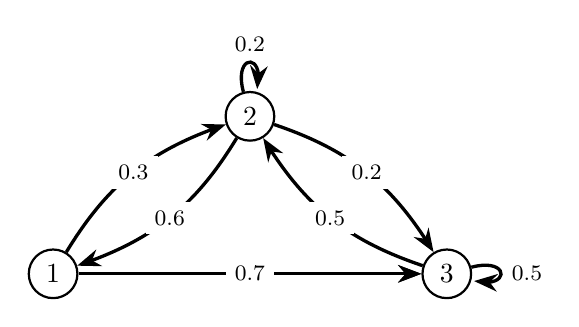
\begin{tikzpicture}
\begin{scope}[every node/.style={circle,thick,draw}]
    \node (A) at (0,0) {1};
    \node (B) at (2.5,2) {2};
    \node (C) at (5,0) {3};

    \end{scope}

\begin{scope}[>={Stealth[black]},
              every node/.style={fill=white,rectangle},
              every edge/.style={draw=black,very thick}]
    \path [->] (A) edge [bend left=20] node[pos=0.5] {\footnotesize{0.3}} (B);
    \path [->] (B) edge [bend left=20] node[pos=0.5] {\footnotesize{0.6}} (A);
    \path [->] (B) edge [bend left=20] node[pos=0.5] {\footnotesize{0.2}} (C);
    \path [->] (C) edge [bend left=20] node[pos=0.5] {\footnotesize{0.5}} (B);
    \path [->] (A) edge (C);
    \path [->] (A) edge node[pos=0.5] {\footnotesize{0.7}} (C);
    \path[<->] (C) edge [loop right] node {\footnotesize{0.5}} ();
    \path[<->] (B) edge [loop above] node {\footnotesize{0.2}} ();
    
    \end{scope}

\end{tikzpicture}
\end{center}


% \begin{equation} \label{eq8}
% \begin{split}
% N_{open1}^{i+1} &=  e^{-\Delta t / \tau_{open}}N_{open1}^{i} + \pr{1 - e^{-\Delta t P_{total}}}N_{closed}^{i} \\ 
% N_{open2}^{i+1} &= \pr{1 - e^{-\Delta t P_{total}}}N_{open2}^{i} + P_{P}\pr{1-e^{-\Delta t / \tau_{open}}}N_{open1}^{i} \\ 
% N_{inactive}^{i+1} &= e^{-\Delta t / \tau_{inact}}N_{inactive}^{i} + \pr{1-P_{P}}\pr{1-e^{-\Delta t / \tau_{open}}}N_{open1}^{i} + e^{-\Delta t P_{P}}N_{open2}^{i}\\
% N_{closed}^{i+1} &= e^{-\Delta t P_{total}}N_{closed}^{i} + \pr{1-e^{\Delta t / \tau_{inact}}}N_{inactive}^{i} \\
% \end{split}
% \end{equation}


Transition matrix: 
\begin{align}
\mathrm{A} =
\begin{bmatrix} %%%%%%%%%%%%%%
0           &  0.3          & 0.7 \\ 
0.6         &  0.2          & 0.2     \\
0           &   0.5         & 0.5    \\ 
\end{bmatrix}
\end{align}

\chapter{Neuron Modeling}

\section{Hodgkin-Huxley} 

\subsection{The Main Form} The pair won the nobel prize for this model, which formed the basis of our understanding of action potentials. Beyond neurons, it was used in modeling pacemakers of the heart, and muscle cell depolarizations before better models existed.  The basis is simply KCL: 

\bigskip

\begin{equation} \label{eq8}
\begin{split}
C\dot{V} = I - I_{Na} - I_{K} - I_{Leak}
\end{split}
\end{equation}

\bigskip

Because the equations can be found in nearly any textbook\footnote{Izhikevich, \textit{Dynamical Systems Neuroscience}} or Wikipedia page, I will focus on some of the conceptual understanding I had issues with at first. The complete equation Hodgkin and Huxley arrived at is as follows: 

\bigskip

\begin{equation} \label{eq8}
\begin{split}
C\dot{V} = I - \bar{g}_{Na}m^3h(V - E_{Na}) - \bar{g}_{K}n^4(V - E_{K}) - \bar{g}_{L}(V - E_{L})
\end{split}
\end{equation}

\bigskip 

There are a few main points to make here. Firstly, this model considers only 3 currents. $Na$ and $K$ are self explanatory, but $Leak$ represents the small amount of current that will always occur in cells due to the many routes of charged particles passing through the membrane. It is restorative, in that it pushes the membrane potential back to the resting voltage.\newline

\subsection{Gating and Conductance} The $\bar{g}$ represent the maximal conductance of these ions. But, shouldn't conductance be variable, depending on how many channels are open? Yes, that is what $m$, $h$, and $n$ are for. These three variables are effectively kinetic fits of the opening and closing dynamics of sodium and potassium channels. Again, I will not mention these equations explicitly as they can be found anywhere. Conceptually, there are three things to know:\newline

Firstly, $m$ is an activation curve for sodium, and the power to the 3rd represents that there are three activation gates. $h$ is an inactivation gate for sodium. Potassium has 4 activation gates, $n$, and no inactivation gate. Gating can be any number of things, for example, $h$ could be a conformtional change that occurs in the channel after it has been open for $0.1 ms$ that closes it again. Naturally, the gating for every channel will be different. Because the $Leak$ current is an ensemble of many channel types, it will not have "gating" per se.\newline

Secondly, $m$, $h$, and $n$ all are between 0 and 1 and represent the \textbf{proportion of channels open}. For instance, if $n = 1$, then 100\% of potassium channels will be open. This is why we multiply by the maximal conductance.\newline

Thirdly, $m$, $h$, and $n$ are dependent upon voltage, which affords them a time constant $\tau$. This is the conceptually most difficult part. The experimental explanation may be beneficial in understanding. Hodgkin and Huxley realized that these three gating variables will converge to different values depending on the voltage. This makes sense, because we know potassium channels are voltage gated, we would expect the gating variable $n$ to converge to around 1 as the voltage increases. But, the rate at which channels open and close is different. Therefore, their experiments were done to vary the voltage and determine how long it took the conductance of the channels to converge to some value. Does this make sense? In simplest terms: channels open and close at different rates, and that depends on the voltage.\newline

What is the implication of this? Again, look up the exact equations if you are interested. Otherwise, trust the following: $m$ has a time constant $\tau_m$ which is very small compared to $\tau_h$ and $\tau_n$. Meaning, sodium channels will open the fastest in response to a voltage increase, causing depolarization of the cell. After some delay, sodium channel inactivation ($h$) and potassium channel activation ($n$) will kick in, causing repolarization and then hyperpolarization. 

\subsubsection{These are all derivatives.}
One of the most difficult conceptual understandings I had was that $\dot{V}$, $m$, $h$, and $n$ are all rates that depend on different time constants, which take voltage as their input. So, the derivative of voltage depends on the derivative of $m$, $h$, and $n$, which depend on voltage. The cyclic nature of this makes it strange, but still doable. Use the general form of derivative, $x_{i+2} = x_{i+1} + (x_{i+1} - x_i)/t$, follow the math, and you will survive.

\section{Fitzhugh-Nagumo Reduction}

\subsection{Why would we simplify this system?} Reduction implies we are reducing the amount of variables. But why would we do this? The system is already incredibly generalized. We only consider two ion channels and are looking at a static neuron. How can we be accurate if we simplify this system any further?\newline

Let's start by doing a simple thought experiment regarding the previous model: 

\bigskip

\begin{center}

    $C\dot{V} = I - \bar{g}_{Na}m^3h(V - E_{Na}) - \bar{g}_{K}n^4(V - E_{K}) - \bar{g}_{L}(V - E_{L})$
    
\end{center}

\bigskip

As mentioned, $m$, $h$, and $n$ have their own time constants $\tau_{m,h,n}$. That means you'll need to do at least 6 calculations in order to determine $\dot{V}$, which, because it is a derivative, has its own time constant $\tau_v$. Thus, the whole equation is $4^{th}$ dimensional with respect to time and requires at least 7 or so calculations per time step. If you'd like to simulate an action potential for around 10ms with a time step of 0.01ms, that means you'll perform around 7,000 calculations. Which is not so bad!\newline 

However, let's say you want to attempt a propagating action potential. Many people would model this on an infinitely long neuron/wire, but for the sake of this thought experiment let's say you're just interested in a 1 cm neuron/wire for 10 ms. To account for this spatial consideration, you'll need to add in another term besides $I$ which receives current input from the previous segment of the neuron. So, this brings us up to at least 8,000 calculations.\newline

You'd probably want to divide up the neuron into segments on the order of 1 $\mu$m. This multiplies our 8,000 calculations by an additional 100,000, giving us 800,000,000 to worry about. Still, this is not horrendous. But, this considers a 1D wire. Neurons are 3D dimensional. We are already considering a system that is $4^{\mathrm{th}}$ dimensional with respect to time, and now we desire to consider $3^{\mathrm{rd}}$ dimensional with respect to space. Imagine trying to calculate the flux through a $1000 \times 1000 \times 1000$ resolution box (i.e., perhaps $\mu m^3$ with good resolution). The surface area of this box is thus $6\times 10^6$. Now extend this surface area to include the length of the wire and the area of the soma and dendrites, giving you thousands of millions of points to calculate per time iteration. And, we are still only considering two ion channels. Neurons have dozens and dozens of channels all with different gating kinetics. It does not consider things like lateral inhibition, birufcation, dendritic input, etc. I'll not bother telling you how many calculations we need to perform beyond this point---but it would be large. 

\subsection{How to Reduce} What do we know about the time constants mentioned in the previous section? Roughly speaking, some are fast and some are slow. The upswing of an action potential is on a fast time constant, and the repolarization is on a slow time constant. We also know that the upswing portion is roughly a positive feedback loop, so as voltage increases, so should the derivative of voltage.\newline

This helps us arrive at least at the following: 

\begin{equation} \label{eq8}
\begin{split}
\dot{V} &= V \times f(x)
\end{split}
\end{equation}


Simply meaning that the derivative should scale with voltage in some way. We also know that there are at least two ``equilibrium points" in a neuron. Meaning, when the neuron is at rest, the $\dot{V}$ will be zero. And, when the neuron reaches the peak of the action potential, the same is true. This will allow us to immediately assume something interesting:

\begin{equation} \label{eq8}
\begin{split}
\dot{V} &= V(V - V_{rest})(V - V_{max})
\end{split}
\end{equation}

We are already almost there. What we have just done is said that when either $V = V_{rest}$ or $V = V_{max}$, the $\dot{V}$ will not change. These are all on the aforementioned ``fast" time scale, and as this is representative of the activation of the action potential, it is effectively a simplification of the sodium channel dynamics. This is also extremely easy to measure experimentally.\newline

On our second time scale, the slow time scale, we have the inactivation/repolarization function. How will this look like? Just as with the first equation, we will want this curve to increase in magnitude with voltage. Because $n$ represented the potassium channel activation in the previous segment, we can use that as our repolarization function here. 

\begin{equation} \label{eq8}
\begin{split}
\dot{n} &= V - \gamma n
\end{split}
\end{equation}

What does this say? It says that our repolarization curve $\dot{n}$ will increase with respect to voltage. But, it will also decrease with respect to itself according to some scaling factor $\gamma$.\newline

Now we have reduced our function down to two dimensions and can combine terms: 
    
\begin{equation} \label{eq8}
\begin{split}
    \dot{V} &= V(V - V_{rest})(V - V_{max}) - n\\ 
    \dot{n} &= V - \gamma n\\
\end{split}
\end{equation}

But, we still want voltage to be affected by an injected current, so we can simply add this term back in. And it is also in this equation that we will add our spatial dependence to reach the following: 

\begin{equation} \label{eq8}
\begin{split}
    \dot{V} &= I_{app} + [V(V - V_{rest})(V - V_{max}) - n] +  D\frac{\partial V^2}{\partial x^2}\\
\end{split}
\end{equation}

$D$ is our spatial dependence, which represents the diffusion of charge around the neuron membrane. And that's it, for now! 

\subsubsection{Circuits digression.}
A lot of the original work done by Fitzhugh and Nagumo used circuit equivalents in order to model neurons. One such example is as follows\footnote{This circuit is adapted from {\textit{Mathematical Physiology}}, by James Keener \& James Sneyd (1998).}:

\begin{center}
 \begin{circuitikz} 
 \draw
    (0, 0) node[op amp,yscale=-1] (opamp) {}
    (opamp.+) to[short] ++(-1,0) 
    to[C] ++(0,1.5)
    (opamp.+) to[short] ++(-1,0)
    to[R] ++(0,-1.5)
    to ++(0,0) node[ground]{}
    (opamp.-) to[short] ++(0,-1) coordinate (leftS)
    to[short] (leftS -| opamp.out)
    to[short] (opamp.out)
    to[R] ++(0,2)
    (-4,2) -- (2,2)
    (-4,2) to[C] (-4,0)
    to ++(0,0) node[ground]{}
    (3.5, 0.5) node[op amp,yscale=-1] (opamp) {}
    (opamp.+) to[short] ++(-0.5,0) 
    to[short] ++(0,1)
    (opamp.-) to[short] ++(-0.5,0) 
    to[short] ++(0,-1)
    to[R] ++(0,-2)
    to ++(0,0) node[ground]{}
    (1.81,-1) to[R] (4.7,-1)
    to[short] (opamp.out)
    to[short] ++(0,1.5)
    to[R] ++(-3,0)
;
\end{circuitikz}

\end{center}

The rightward opamp functions as a Schmitt Trigger, and the entire thing is effectively an opamp oscillator with a second opamp in the middle. The purpose is to simulate an excitable system, like a neuron that is continually firing. Excitable systems systems are those that fire and have some refractory period before firing again (for example forest fires, or even your toilet).


\section{Diffusion}

 Note that in the coming sections, $[f]$ is used to describe the concentration of some molecule $f$. But, this principal can be applied to anything, including the spreading of voltage across some surface. 

\subsection{Forward Euler's} Diffusion is accomplished using some diffusion coefficient ($D_c$) multiplied by some measure of the proportion in one compartment verses another (often $\partial^2 [f]/\partial x^2)$. $D_c$ can be tuned however desired. The important bit is the second derivative of $[f]$ with respect to space. This can be done using the general form of a second derivative, as written below: 

\begin{equation} \label{diff1}
\begin{split}
f'' = \frac{f_{x + 1} - 2f_x + f_{x - 1}}{x^2}
\end{split}
\end{equation}

\bigskip

One may wonder how one would solve for an edge case, as the general form of a second derivative requires three data points. There are some nuances, but in general the solution is simply the first derivative of the non-edge side. That is, since the second derivative is the difference in derivatives, that leaves simply the derivative of one side minus zero. This is like applying a closed end to your surface. You can ponder how to solve for an open end, if that ever arises.\newline

This method has some slight issues in which the $[f]$ can occasionally go negative. The way in which this occurs is stated below (note that now $[f]$ is used instead of $f$ to signify concentration at a value $x$ and time $t$). We can first describe a simplified version of the problem:

\begin{equation} \label{eq8}
\begin{split}
[f]_i & = f_0\exp(-mt) \\
\frac{d[f]}{dt} & = \frac{[f]_{i+1} - [f]_{i}}{\Delta t} = -m[f]_i \\
[f]_{i+1} & = (1-m\Delta t)[f]_i = [f]_i - m\Delta t [f]_i \\
[f]_{i} & = (1-m\Delta t)[f]_{i-1} = (1-m\Delta t)^2[f]_{i-2} \\
[f]_{i} & = (1-m\Delta t)^i[f]_{0} \\
\end{split}
\end{equation}

You can see easily, from this, that if $\Delta t$ is too big, you will abandon the characteristic decay you'd expect from $f_0\exp(-mt)$, and instead get some diverging oscillatory function. How this applies to our interest in diffusion is described below: 

\begin{equation} \label{eq8}
\begin{split}
\frac{[f]^{t+1}_{x} - [f]^{t}_{x}}{\Delta t} &= \frac{[f]^{t}_{x+1} - 2[f]^{t}_x + [f]^{t}_{x - 1}}{x^2}\\
[f]^{t+1}_{x} - [f]^{t}_{x} &= \frac{\Delta t}{x^2} \pr{[f]^{t}_{x+1} - 2[f]^{t}_x + [f]^{t}_{x - 1}} \\
[f]^{t+1}_{x} &= \frac{\Delta t}{x^2} [f]^{t}_{x+1} + \pr{1 - 2\frac{\Delta t}{x^2}}[f]^{t}_x + \frac{\Delta t}{x^2}[f]^{t}_{x - 1} \\
\end{split}
\end{equation}

Therefore, if we want to ensure that the concentration is always positive, we are constrained by: 

\begin{equation} \label{eq8}
\begin{split}
1 - 2\frac{\Delta t}{x^2} & = 0\\
\Delta t & < \frac{x^2}{2}\\
\end{split}
\end{equation}

The relevance of this being that if one were interested in modeling on a very small $\Delta x$, then one would have to use a $\Delta t$ that is not physiological, and thus waste a great deal of computing power in doing so. This can be avoided explicitly using some other methods, discussed next. 

\subsection{Backward Euler's} This form serves to solve the time-scale dilemma by swapping $[f]_{x+1}$, and can be used with any $\Delta t$. Let us consider the same example from above: 

\begin{equation} \label{eq8}
\begin{split}
[f]_i & = f_0\exp(-mt) \\
\frac{d[f]}{dt} & = \frac{[f]_{i+1} - [f]_{i}}{\Delta t} = -m[f]_{i+1} \\
[f]_{i+1} - [f]_{i} & = -m\Delta t[f]_{i+1} \\
[f]_{i+1} & = \frac{1}{1+m\Delta t}[f]_{i} \\
\end{split}
\end{equation}

Naturally, there is no longer a concern of the size of $\Delta t$. Though, one immediate concern is the difficulty of solving your equation for $[f]_{i+1}$. Getting back to the diffusion interest, we now have:

\begin{equation} \label{eq8}
\begin{split}
\frac{[f]^{t+1}_{x} - [f]^{t}_{x}}{\Delta t} &= \frac{[f]^{t+1}_{x+1} - 2[f]^{t+1}_x + [f]^{t+1}_{x - 1}}{x^2}\\
[f]^{t+1}_{x} - [f]^{t}_{x} &= \frac{\Delta t}{x^2} \pr{[f]^{t+1}_{x+1} - 2[f]^{t}_x + [f]^{t-1}_{x - 1}} \\
\end{split}
\end{equation}


Which simply replaces the previous $[f]^{t}_{x}$ with $[f]^{t+1}_{x}$. This leaves us with three unknowns (those being $[f]^{t+1}$ at $x-1,x,x+1$). We must use linear algebra to solve by first rewriting the left and right side as vectors and a matrix in the following way: 

\begin{align}
\vec{[f]}^{t+1} &= \begin{bmatrix}
        [f]^{t+1}_{0} \\
        [f]^{t+1}_{1} \\
        \vdots \\
        [f]^{t+1}_{x}
\end{bmatrix}
; \vec{[f]}^{t} = \begin{bmatrix}
        [f]^{t}_{0} \\
        [f]^{t}_{1} \\
        \vdots \\
        [f]^{t}_{x}
\end{bmatrix}
\end{align}

and 
\begin{align}
\mathrm{A} = \frac{\Delta t}{x^2}
\begin{bmatrix} %%%%%%%%%%%%%%
\dots       &   \dots       & \dots     &   \dots    &   \dots   \\
1           &   -2          & 1         &            &   \vdots    \\
\vdots      &   1           & -2        &   1        &   \vdots   \\   
\vdots      &               & 1         &   -2       &   1    \\
\dots       &   \dots       & \dots     &   \dots    &   \dots    \\
\end{bmatrix}
\end{align}

The corners $1,1$ and $x,x$ were intentionally omitted, as what one desires to do with this is dependent on how they would prefer to treat their edges. As described before in the \textit{Forward Euler's} method, one can use instead of the $(1,-2,1)$ pattern, simply $(\varnothing,-1,1)$ pattern, which signifies a closed edge. Therefore, together now we get: 

\begin{equation} \label{eq8}
\begin{split}
\vec{[f]}^{t+1} - \vec{[f]}^{t} & = \mathrm{A} \vec{[f]}^{t+1} \\
\mathrm{I}\vec{[f]}^{t+1} - \mathrm{A}\vec{[f]}^{t+1} & = \vec{[f]}^{t} \\
\vec{[f]}^{t+1} & = (\mathrm{I} - \mathrm{A})^{-1}\vec{[f]}^{t}
\end{split}
\end{equation}

Where I is the identity matrix. 

\subsubsection{Remarks.} 
Foward Euler's is explicit, and will be preferred whenever the differential equations are non-stiff\footnote{On approximately the same time scale.}. It is the more accurate of the two methods, and can be less computationally intensive if your decay rates are all slow. Backward Euler's is implicit, and can not be used to solve everything, but is doable in most cases. The extra computation required to solve the system of equations more than makes up for potential limitations in your $\Delta t$. 

\subsubsection{Ramblings.} 
I have this constant wonder if this method can be used to model the spread of voltage over a resistor lattice, by perfecting the $D_c$ value. I am presuming it would work for a sufficiently large lattice, perhaps $100 \times 100$. This would be a good exercise to do sometime in the future. 



\chapter{Modeling Circuits}
\label{Modeling Circuits}

The idea of this algorithm comes from\footnote{\url{https://lpsa.swarthmore.edu/Systems/Electrical/mna/MNA3.html}} and is an expansion of what was discussed earlier in the \textbf{Electronics} part of this book. Not by coincidence, both of the examples in the earlier section had symmetric matrices. The general way to extract equations from a circuit is in the following pattern:   

\begin{align}
\begin{bmatrix} 
\mathrm{G} &   \V \\
\V^T   &   \mathrm{Z}  \\
\end{bmatrix}
\end{align}

G is essentially the way nodes are connected by resistors (represented as conductances). The diagonal represents the total number of resistors connected to a diagonal, and the other bits represents how nodes are connected by resistors. I will use the example provided in the footnote directly to illustrate: 

\begin{center}
\begin{circuitikz}[american]
\draw 

(-3,-1) to [battery,l_=$V_{s1}$] (-5,-1)
(-5,-1) to [R,l_=$R_1$] (-5,-3)
(-5,-3) -- (-3,-3)

(-1,-1) to [battery,l=$V_{s2}$] (-1,-3)
(-1,-1) to [R,l_=$R_2$] (-3,-1)
(-3,-1) to [R,l_=$R_3$] (-3,-3)
(-3,-1) to [short, *-] (-3,-1)
(-1,-1) to [short, *-] (-1,-1)
(-3,-3) to [short, *-] (-3,-3)
(-5,-0.55) node {$V_1$}
(-3,-0.55) node {$V_2$}
(-1,-0.55) node {$V_3$}
(-2.7,-2.7) node {$V_4$}
(-5,-1) to [short, *-] (-5,-1)
(-1,-3) -- (-3,-3)
to ++(0,0) node[ground]{};

\end{circuitikz}
\end{center}

There are 4 nodes, but as mentioned before, Node 4 is grounded, a reference, and thus not included in our calculations. This will mean our matrix G must be $n \times n$, where $n$ is $N - 1$. Node 1 is connected only to $R_1$, resolving the $(0,0)$\footnote{You are a computer scientist in addition to a mathematician, so of course our matricies must be 0 indexed.} position of the matrix to be $G_1$. Node 2 is connected to $R_2$ and $R_3$, giving us $(1,1) = G_2 + G_3$. Node 3 to only $R_3$, giving us $(2,2) = G_3$. Node 2 and Node 3 are connected via $R_2$, meaning the $1,2$ and $2,1$ positions will have a $G_2$, though notably, it will be $-G_2$:

\begin{align}
\mathrm{G} = 
\begin{bmatrix} 
G_1 & 0 & 0 \\
0 & G_2 + G_3 & -G_2 \\
0 & -G_2 & G_2 \\
\end{bmatrix}
\end{align}

There are two voltage sources ($V = 2$), and 3 nodes, meaning the matrix must be $n \times m$, where $n = N-1$ and $m = V$. You fill the matrix as if the positive terminal of the $j^{\mathrm{th}}$ voltage source is connected to the $i^{\mathrm{th}}$ node, point $(i,j) = 1$, or $(i,j) = -1$ for the negative terminal. So for the above, since the negative terminal of $V_{s1}$ is connected to Node 1, $(0,0) = -1$, and as the positive terminal connects to Node 2, $(1,0) = 1$. Lastly, as Node 3 connects to the positive terminal of $V_{s1}$, $(2,1) = 1$. 
\begin{multicols}{2}
\begin{align}
\mathrm{V} = 
\begin{bmatrix} 
-1 & 0 \\
1 & 0  \\
0 & 1  \\
\end{bmatrix}
\end{align}

\begin{align}
\mathrm{V}^T = 
\begin{bmatrix} 
-1 & 1 & 0 \\
0 & 0  & 1 \\
\end{bmatrix}
\end{align}
\end{multicols}

And lastly, Z for zero is an $n \times n$ matrix of zeros where $n = V$:

\begin{align}
\mathrm{V}^T = 
\begin{bmatrix} 
0 & 0  \\
0 & 0   \\
\end{bmatrix}
\end{align}

Giving us an $\mathrm{A}x = \mathrm{B}$ of: 

\begin{align}
\begin{bmatrix} 
G_1 & 0 & 0 & -1 & 0 \\
0 & G_2 + G_3 & -G_2 & 1 & 0  \\
0 & -G_2 & G_2 & 0 & 1  \\
-1 & 1 & 0 & 0 & 0  \\
0 & 0  & 1 & 0 & 0  \\
\end{bmatrix}
\begin{bmatrix} 
V_1 \\
V_2  \\
V_3  \\
I_1  \\
I_3 \\
\end{bmatrix}
=
\begin{bmatrix} 
0 \\
0  \\
0  \\
V_{s1}  \\
V_{s2} \\
\end{bmatrix}
\end{align}

You may, rightfully, say ``\textit{Uh, who cares?}," since we arleady know that each row corresponds to a different equation. Well, there are a few reasons. Firstly, doing this algorithmically allows us to avoid accidentally underdetermining our matrix using the ol' eye-balling it technique. More importantly, though, the algorithmic approach allows us to solve this via code. Once I can write a bit more neatly, I'll likely upload some snippets here. 

\part[Physiology]{Physiology
            \vspace{0.2in}
            \begin{center}
            \begin{minipage}[l]{10cm}\small
                Preoccupied with a single leaf, you won't see the tree. Preoccupied with a single tree, you'll miss the entire forest.  \newline
                -- Vagabond by Takehiko Inoue
            \end{minipage}
            \end{center}}

\section{Perspective}

It is very important to avoid taking a quantized approach to studying physiology. You'll notice neuroscience majors may know some superb nuances regarding the role of HCN channels in overexcitable neural disorders, like epilepsy. However, they may be totally unaware of their canonical role as pacemakers in the heart. So too may they be unaware of the rich history of modeling $I_h$ currents by computational biologists, preferring to look only at a channel as it functions in neurons and is testable in a cell culture. Hence, one must not become preoccupied with a single leaf.\newline

Another bit of wisdom comes from Yoshikawa's Musashi. There is a chapter in which vagabonds are tilling a marsh's untenable land. Each time a storm came, all work was reset as flooding returned the land to mud. One realized that they had been tilling the field in the shape of a square, unconsciously aiming for a uniform, symmetrical crop that is typical of any farm. In doing so, they intended to bend nature from its gruff state into something it was not. Nature, not allowing this, cyclically reclaimed the land. But, if they tilled the land in an oblong fashion, asymmetrical and with the natural bends of the marsh, along the path that water would flow in a storm---perhaps the fields would survive the storm. Rather than trying to oppose the universe, one must first know its way, and be guided by it.\newline

Surgical intervention is most often an opposition to the way of nature. Indeed, the most clear evidence of this is in today's BSIs which attempt to escape endogenous circuits all together. Perhaps one should focus more on enhancing nature's way first, before opposing it. And to enhance nature's way, one must understand it fully. 

\chapter{Biochemistry}

To be able to interface with the electrophysiology of neurons, one must fully understand it. 

\section{Ion Channels}


This section will be filled in better throughout the semester, through more Biochem courses. 


\chapter{Muscles}

A large part of this information comes from Dee Silverthorn's \textit{Human Physiology} textbook---arguably the best textbook of all time. 

\section{Skeletal Muscle}
\subsection{A Cellular Level}
\subsubsection{Structure.}
Skeletal muscles are composed of muscle fibers, which are composed of myofibrils. Muscles use a silly nomenclature, in which ``sarco" is added to words. For example, the whole structure sits within the sarcoplasm (cytoplasm), fibers are intertwined with the the sarcoplasmic reticulum (equivalent to endoplasmic reticulum) and surrounded by the sarcolemma (equivalent to the cell membrane). An individual myofibril is made up of overlapping actin and myosin segments, held together, to some degree, by titin. The myosin heads are the canonical structure you imagine, which bud off of the end of a chain like leaves on a branch and bind to actin. Undeniably, the most uninteresting part of muscle physiology is as follows: The ``centerline" of the myosin networks is called the M line, while the ``centerline" of the actin network is called a Z disk. Titin branches off from the Z disks to bind to the ends of myosin chains, providing both some elasticity and support for myosin. Actin chains are centered around a line of nebulin, which too provides structural support and organization. The I band is considered to be the unbound part of the actin structure, centered around the Z disks. The H zone is the unbound part of the myosin structure, centered around the M line. The A band is the entire length of the myosin fibers, thereby encapsulating both the bound part of the actin-myosin complex and the H zone, meaning it too is centered around the M line. Therefore, when contraction occurs, the size of the H zone and I band decreases, while the size of the A band stays the same.

\subsubsection{Contraction-relaxation.}
Myosin heads desire to bind to actin, but are blocked by tropomyosin. Ca$^{2+}$ can bind to troponin, bound to tropomyosin, to cause conformational changes resulting in the exposure of the actin to the myosin heads. In doing so, binding can occur, followed by myosin's power stroke. The energy for the stroke comes from hydrolyzing ATP, which had already occured by the time myosin attached to the actin. The powerstroke allows the release of the ADP and P$_i$. ATP then can bind to the empty active site of myosin, which causes the release of the head and prepares it for another cycle. Notably, when ATP does not bind to myosin, the muscle will be stuck in the rigor state.\newline

In skeletal muscles, the source of Ca$^{2+}$ is a combination of the extracellular Ca$^{2+}$ flowing inward, and further release from the sarcoplasmic reticulum. The story goes as follows: a motor neuron releases acetylcholine onto the motor end plate (an area which a high density of sodium channels). This causes a depolarization, which propagates down the muscle fiber. Structures called T-tubulues sink lower into the tissue, allowing for more direct access to the inner processes (visually, these look similar to gyri in the brain or the crypts of the intestinal wall). The T-tubules are lined with dihyropyridine (DHP) channels, an L-type VGCC (specifically Ca$_v$1.1). DHP and ryanodine receptors (RyR) can be mechanically coupled, which influx of Ca$^{2+}$ in through DHP mechanically opens RyR channels of the sarcoplasmic reticulum (a large store of Ca$^{2+}$). The free calcium is lowered through things like active pumping out of the sarcoplasm.\newline

A steady supply of ATP is needed to maintain pumping, and it is said that at any given time, there is 8 or so twitches worth of ATP within the muscle fiber. Therefore, frequent production and alternate stores are required for continuous movement. One such storage is phosphocreatine, whose phosphate group can be quickly transferred to ADP through creatine kinase. Muscles therefore contain high levels of this enzyme, and \textbf{testing for it in the bloodstream can be a good proxy for muscle damage}.\newline

Notably, it is very difficult to fully deplete a muscle of its ATP. Other forms of fatigue begin before this can possibly occur, which include CNS or PNS feedback. An example of this may be that acetylcholine is not synthesized fast enough to continually stimulate muscle fibers. Continual simulation of muscle fibers, beyond what is allowable under normal conditions, \textbf{will fully deplete ATP levels and therefore cause damage to muscles}. Another consideration is the continuous use of ATP may result in P$_i$ buildup in the sarcoplasm, making release of ADP $+$ P$_i$ from myosin less likely to occur. Too, this opens the possibility of calcium phosphate forming, which can be quite damaging if it crystallizes further. There are also ion concentration changes to consider, and continued stimulation can result it tetanus.

\subsubsection{Disorders Digression.}
There are many ways one can lose control of their muscles. Nerve damage, for example, will halt the release of acetylcholine onto the motor plate. In a similar manner, botulism is a result of the botulinum toxin blocking release of acetylcholine, resembling the effect of nerve damage. In muscular dystrophy, the protein dystrophin is absent, which would normally attach actin to the cell membrane. Evidently, this can result in membrane permeability, calcium influx, and thus activation of digestive enzymes that breakdown muscle fibers. In McArdle's disease, muscles simply cannot convert glycogen to glucose-6-phosphase, causing the energy supply to be limited. 


\section{Smooth Muscle}

Smooth muscle is much more variable than skeletal, differing by location, contraction pattern, required inputs, and structure. 


\subsection{A Cellular Level}
\subsubsection{Structure.}
Smooth muscle is not considered to have sarcomeres, despite it having the same basic structural components of skeletal muscles. Smooth muscle contains much more aactin than does skeletal muscle, and notably does not contain troponin like skeletal muscle does. Smooth muscle networks are connected through intermediate filaments, which usually attach to dense bodies within the cytoplasm. Actin also attaches to dense bodies, maintaining the actin-myosin network within the cell as well. Smooth muscles do not have T-tubules like skeletal muscles. A comparable structure may be calveolae, which do indent into the membrane and seem spatially associated with the sarcoplasmic reticulum. The autonomic nervous system stimulates fibers through neurotransmitter release from varicosities, or bulbous stores of the chemical. The neurons may innervate the muscle fibers, allowing multiple muscle cells to be stimulated at once, or they may be release to a few fibers, which are connected through gap junctions and stimulate the nearby ones, causing a propagating wave to stimulate others. The first case describes a multi-subunit muscle, and the second a single subunit. 

\subsubsection{Contraction-Relaxation.} 
Initiation of contraction begins the same as skeletal muscle, in that calcium enters and the concentration is further driven up by sarcoplasmic calcium release. Though, in this case Ca$^{2+}$ may enter either through gap junctions or membrane ion channels. As such, there are many more modes of entry than in skeletal muscle. For example, voltage-gated Ca$^{2+}$ channels may open, but there are also ligand gated channels or stretch-activated channels, adding extra layers of possible regulation. Intracellular differences arise beginning from release from the SR. Firstly, is is no longer a mechanically gated RyR channel which allows its release. The release mechanism is now Ca$^{2+}$ activated RyR release (commonly called Ca$^{2+}$-induced-Ca$^{2+}$-release (CICR)), and the IP$_3$ path. GPCRs activate phospholipase C, driving IP$_3$ production which binds to SR channels and causes them to open. The IP$_3$ path is usually considered the greatest way to drive up intracellular Ca$^{2+}$ (or at least, that is what computational biologists seem to think). When Ca$^{2+}$ is available, it binds to calmodulin (CaM), which then binds to the myosin light chain kinase (MLCK). MLCK phosphorylates myosin to increase myosin ATPase activity. Importantly, once contraction occurs, it stays stiff until released by a different mechanism. Because after contraction, no work is being done in the stiff state, smooth muscle is able to stay contracted for long periods. This explains why sphincters in the body are able to stay closed all the time, while one's bicep fatigues after carrying groceries for just a little while. Relaxation begins when Ca$^{2+}$ is either pumped out of the cell through a Ca$^{2+}$ATPase pump, or sodium transporter. This causes CaM to unbind, myosin light chain phosphatase (MLCP) to dephosphorylate myosin, and the myosin heads to release from actin. Interestingly, diacylglycerol (DAG), another product of the IP$_3$ path, inhibits MLCP and thereby enhances muscle contraction.\newline

The calcium stored in the SR is maintained in a number of ways. One example being the protein STIM1 responding to lower Ca$^{2+}$ levels within it, moving toward the cell membrane, and activating store operated Ca$^{2+}$ channels, such as Orai1. 

\section{Cardiac Muscle}

\subsection{A Cellular Level}

\subsubsection{Structure.}
Cardiac cells contain sarcomeres, but the fibers themselves are smaller and often mono-nucleated. Cell edges are called \textit{intercalated disks}, held together by desmosomes and permeated by gap junctions. The role of gap junctions is obvious but essential, and key to the rhythmic firing of the heart. Despite not requiring nervous system input, cardiac muscles have large T-tubules, and a significant amount of mitochondria. 

\subsubsection{Contraction-Relaxation.} 

Initiation of cardiac muscle contraction requires extracellular calcium, and generation can be graded. The entrance of Ca$^{2+}$ powers the opening of non-mechanical RyR channels, as a method of CICR. Because of this, the sarcoplasmic reticulum is smaller in the myocardium, because some of the Ca$^{2+}$ required for contraction comes from extracellular entry in about a 10:1 ratio of sarcoplasmic reticulum:extracellular origin. Ca$^{2+}$ is removed using the Na$^+$-Ca$^{2+}$ exchanger (NCX).\newline

The electrophysiological profile is marked by Na$^+$ entry but maintained by Ca$^{2+}$ in a plateau phase. The fall occurs via K$^+$ entry. The refractory period is long due to this plateau phase, which prevents Na$^+$ channels from resetting. 

\subsubsection{Pacemakers.}
Hyperpolarization cyclic nucleotide (HCN) gated channels induce an inward hyperpolarization ($I_h$, or $I_f$) current. Within the hyperpolarization range, HCN channels open and cause steady depolarization rhythmically. HCN channels are typically permeably to multiple cations, and in this case Na$^+$ is the biggest player. When the membrane potential is high enough, VGCCs will open and cause depolarization required to propagate the signal between myocytes. At peak, slow opening K$^+$ channels open and repolarize the membrane. Notably, voltage gated Na channels do not play a role in myocyte depolarization. \newline

Expectedly, as $\beta$-blockers will inhibit a rise in cAMP, HCN channels will be less active. This decreases heart rate, among other things. 


\chapter{Sensory Processing}

Somatic senses are picked up by receptors on \textit{primary sensory neurons}, whose cell bodies reside in the dorsal root ganglia and project to CNS interneurons. Such interneurons are considered \textit{secondary sensory neurons} and they location depends on function. Fast traveling senses, like proprioception, are sent to the medulla before reaching interneurons (cross the body's midline in the brain), while slower traveling senses, like temperature, synapse onto interneurons upon enterring the spinal cord (immediately crossing the midline). Neurons of the thalamus are considered \textit{tertiary sensory neurons} and project to the somatosensory cortex. 


\section{Various Senses}

\subsection{Touch}

\subsection{Temperature}

\subsection{Pain}
Nociceptive neurons respond to a variety of stimuli that can cause damage to cells. Afferent pain signals are carried either by myelinated A$\delta$ and unmyelinated C fibers. A$\delta$ carried pain is faster and perceived as sharp, local pain. C fiber carried pain is less sharp and less localized.\newline

Transient receptor potential (TRP) channels are the most canonical class of ion channels, and are responsible for a great deal of pain sensation. Vanilloid (TRPV$_1$) channels respond to heat, while TRPM8 respond to cold. An immediate response to cell damage is lysing, causing marked increase in K$^+$ in the surrounding areas. Other released chemicals include histamine and prostaglandins. Upon activation, nociceptive neurons can trigger two responses. The first being reflexes that are integrated at the spinal cord, and the second being somatosensory cortex integration\footnote{This ended up being much less interesting to write than I thought it would be.}. 







\chapter{The Spinal Cord}

\section{General Structure}
A cross section of the spinal cord would reveal meninges just like the brain and skull; an outer layer of dura, then arachnoid, and finally pia mater. Too, there is an outer layer of white matter followed by a grey matter interior, which is centered around a ``central canal." The spinal cord has 33 vertebrae, beginning with cervical (C$_1$ to C$_7$), then thoracic (T$_1$ to T$_{12}$), then lumbar (L$_1$ to L$_5$), then sacral (S$_1$ to S$_5$), and finally one coccyx (Co$_1$ to Co$_4$). The sacral, and especially the coccygeal, vertebrae are fused, so you may see them depicted as a single unit. Adding slightly to the confusion is that there are only 31 pairs of spinal nerves. These are C$_1$ - C$_8$, T$_1$ - T$_{12}$, L$_1$ - L$_5$, S$_1$ - S$_5$, and Co$_1$. \textbf{Note: The difference in the nerve location and vertebrae labels is actually quite important, as it is not always that a fracture at some vertebrae leads to nerve damage at the same site}---this is expanded on in later chapters. The spinal nerves exit the spinal cord on either side, i.e., either dorsal or ventral roots. Dorsal entry neurons carry sensory information to the CNS, while ventral exit zones carry information from the CNS to the muscles. Though, importantly, their axons can not necessarily be found on either side, this will depend on where crossing over occurs. The secton of grey matter which connects to the dorsal root is called the dorsal horn, and the same is true for the ventral horn. The lateral horn is in between the dorsal and ventral horns.\newline

\textcolor{red}{Note to self: It might be fun to add a more detailed breakdown at some point, such as the general arrangement of all the nuclei in the spinal cord.}\newline

\textcolor{red}{Another note to self: It would be good to integrate more clinical outcomes into this. For example, what happens in the case of SCI at various vertebrae, or in vagotomy, etc.}

\section{Autonomic Nervous System}
Pathways of the autonomic nervous system require two neurons, one that originates in the CNS and terminates at a ganglion, and a post-ganglionic neuron which terminates at the tissue of interest. While the circuit is often considered to have only two neurons, in fact many pre-ganglionic neurons synapse onto many post-ganglionic neurons, which means one neuron can affect many target tissues. Adding to this is the mode of release. The connection between neuron and target tissue is called the \textit{neuroeffector junction}. At this junction, transmitters are secrete indirectly from bulbous varicosities into the interstitial space, meaning neurotransmitters can diffuse over a larger area. Fascinatingly, these neurotransmitters are actually often synthesized within the axon / varicosities of neurons. 

\subsection{Sympathetic Nervous System}
Pre-ganglionic neurons of the sympathetic nervous system originate in the hypothalamus or reticular formation and extend down to the mid-sections of the spinal cord, from neuron pairs T$_1$ to L$_2$. Sympathetic ganglia are directly beside the spinal cord in a long chain (often called the sympathetic chain). Generally speaking, neurons closer to the T$_1$ section correspond to organs higher in the body, such as the heart or lungs, while neurons closer to the L$_2$ section corresponds to those lower in the body, like one's reproductive organs\footnote{Memorizing which nerves respond to which segments is likely not a good use of your time at this stage..., although it might have some clinical use to know which organs may be affected after SCI.}.\newline

Pre-ganglionic neurons release acetylcholine onto nicotinic receptors,  and post-ganglionic neurons release norepinephrine onto adrenergic receptors. As all adrenergic receptors are GPCRs, their cellular response will be slower than ion channel transmission and occur at the protein-level primarily. Too, they will occur through secondary messenger, for example through the IP$_3$ path or cAMP. Norepinepherine is a tyrosine derivative and, like other catecholamines, can be broken down either by monoamine oxidase (MOA) in the neuron's mitochondria, requiring re-uptake, or in the liver by catechol-o-methyltransferase (COMT).\newline

Dysregulation of the sympathetic nervous system most often manifests as cardiovascular pathologies, such as low blood pressure. Though, incontinence or impotence may also occur. On a cellular level, a process called \textit{denervation hypersistivity} may also occur, where in response to decreased sympathetic neurotransmitters, the body increases expression adrenergic receptors. This is easily measured as increased response from small doses of norepinephrine. 

\subsubsection{Adrenal Medulla Digression.} 
It's worth noting that the adrenal medulla secretes epinephrine in a hormone-like manner. However, the adrenal medulla is often considered a collection of pre-ganglionic neurons, meaning epinepherine acts globally like a hormone, but is also a neurotransmitter.\newline

Let us look at the different adrenergic receptors\footnote{This is ripped directly from Silverthorn.}: 

\begin{table}[!htbp]
\centering
\begin{tabular}{*5c}
\toprule
{} &  \multicolumn{2}{c}{Adrenergic Receptors} & \\
\midrule
{Receptor}   & Location & Sensitivity & Effect \\
\midrule
$\alpha_1$  &  Most tissues & NE $>$ E & Increase Ca$^{2+}$   \\
$\alpha_2$  &  Gut and pancreas & NE $>$ E & Decrease cAMP  \\
$\beta_1$   &  Heart and kidney  &  NE $=$ E & Increase cAMP   \\
$\beta_2$   &  Select smooth muscle  &  NE $<$ E & Increase cAMP   \\
$\beta_3$  &  Adipose  & NE $>$ E & Increase cAMP   \\
\bottomrule
\end{tabular}
\end{table}

\subsection{Paraympathetic Nervous System}
Parasympathetic neurons originate from the uppermost and lowermost neurons, either leaving directly from the cranial nerves or from the S$_2$ to S$_4$ nerves. Ganglia in the parasympathetic nervous system are close to the target tissue, meaning post-ganglionic neurons are very short compared to the pre-ganglionic ones. One of the most paths being from the vagus nerve (a cranial nerve) that carries the majority of parasympathetic signals to organs including the heart, lungs, liver, stomach, intestines, and pancreas. Like the sympathetic nervous system, pre-ganglionic neurons release acetylcholine onto nicotinic receptors. Notably, parasympathetic post-ganglionic neurons also secrete acetylcholine, but onto muscarinic receptors instead. 


\begin{table}[!htbp]
\centering
\begin{tabular}{*5c}
\toprule
{} &  \multicolumn{2}{c}{Cholingergic Receptors} & {}\\
\midrule
{Receptor}   & Location & Effect \\
\midrule
N$_N$  &  Postganglionic neurons & Opens cation channels   \\
N$_M$  &  Skeletal muscle  & Opens cation channels  \\
M$_1$, M$_3$, M$_5$   &  Target tissues   & Increase Ca$^{2+}$   \\
M$_2$, M$_4$   &  Target tissues   & Decrease cAMP, open K$^+$ channels   \\
\bottomrule
\end{tabular}
\end{table}


\subsubsection{Exceptions.}
There are some exceptions to these rules, such as some sympathetic postganglionic neurons that terminate on sweat glands secrete norepinepherine rather than acetylcholine. These are called ``sympathetic cholinergic neurons." There are also neurons which secrete none of these, are are called ``nonadrenergic, noncholingeric neurons." There are also neurons which secrete multiple types of neurotransmitters. 

\section{Somatic Nervous System}
The somatic motor division is exclusively excitatory, and neurons project from the CNS all the way to muscles. Inhibition can occur at the neuronal level (i.e., motor neurons are inibited) but not at the muscle level. Cell bodies of motor neurons are either within the ventral horn of the spinal cord or within the brain. Close to the muscle itself, the axons branches and connects to the muscle at the neuromuscular junction (NMJ), which includes both the target muscle and Schwann cell projections. The ``synapse" equivalent is called the \textit{motor end plate}, which is an area on the muscle with a high density of nicotinic receptors. The ECM contains acetylcholinesterase, responsible for breaking down acetylcholine. Notably, the nicotinic receptors on muscle cells are considered N$_M$, a slightly different version than is found on neurons (N$_N$). This difference has proven to be curical in examples such as $\alpha$-bungarotoxin, which binds only to N$_M$\footnote{Dee Silverthorn quite possibly wrote the greatest textbook known to humanity, didn't she?}.

\section{Acetylcholine, Nicotinic Receptors, and Muscarinic Receptors}

Acetylcholine (which I'll call ACh for this section) is unquestionably one of the most important molecules in the body. It is sythesized from choline (a hydroxyl azanium) and acetyl-CoA. Typical usage goes as follows: ACh is released from vesicles and binds to cholinergic receptors. Upon unbinding, acetylcholinesterase (AChE) breaks it down into acetate and choline. Choline is brought back into the pre-synaptic neuron through sodium cotransporters so that it may be reused. It is then re-combined with acetyl-CoA and repackaged and vesicles.\newline 

Funnily enough, nicotinic receptors (nAChRs) have been described as the most well understood membrane receptor\footnote{\url{https://www.nature.com/articles/nrd2927}}. Nicotinic receptors are fast opening non-specific cationic channels.  They are expressed throughout much of the major structures in the brain, peripheral nervous system, and skeletal muscle. As such, drugs targeting these receptors are of considerable interest in many neurological disorders. The binding site for ACh is composed of aromatic amino acids, namely W and Y. This paper describes continual exposure to drugs treating nAChRs as causing their eventual desensitization, while exposure to nicotine increases their expression greatly.\newline

Both of these are of key interest in treating Alzheimer's disease, as loss of cholinergic synapses is one of its features (including significant reduction of both muscarinic and nicotinic receptors). Interestingly, Alzheimer's shows varying loss of nicotinic receptor subtypes across the brain. There is no shortage of drugs currently in development for reversing this.\newline

\subsubsection{Myasthena Gravis Digression.}
Myasthena Gravis, an autoimmune disorder, is an example of an actylcholine dysregulation caused muscle disorder. As a digression within a digression, autoimmune disorders most often target endocrine organs, and the belief is that they are to protect against mutations causing hypersecretion\footnote{\url{https://www.cell.com/immunity/pdf/S1074-7613(20)30180-1.pdf}}. Upon first glance, you may think that Myasthena Gravis evades this generality, but in fact it does not, as it is well associated with patients that dually have a thymoma (tumor of the thymus). Immune cells begin attacking cells with ACh recepetors, tagging them with antibodies. Therefore, Myasthena Gravis presents itself usually in the weaker muscles, such as those that control the eyes, as they have less ACh receptors and therefore a diminished response to signals. Thus, patients may have drooped eyelids (ptosis), double vision (diplopia), or trouble following moving objects with their eyes. The disease worsens with increased activity, as this causes more antibodies to be released onto ACh receptors---but improves on rest. Fascinatingly, men and women ``get" the disease at different times (women typically under 40, while men over 60).\newline

Antibodies may also target other genes (such as MUSK or LRP4) which are involved in ACh receptor localization, or other forms of regulation.



\section{Central Pattern Generation}

Defining the central pattern generator is still somewhat contested. Computational models have been used to explore its existence\footnote{\url{https://www.nature.com/articles/s41598-021-91714-1}}, and for now we should take a few unifying assumptions: \textbf{(1)} the central pattern generator exists and is used to generate rhythmic moving, such as walking, \textbf{(2)} in many cases it is initiated by the CNS, but aside from that is largely devoid from CNS input, and \textbf{(3)} the CNS can work in tandem to compute integrated moving that requires coordination and balance. 

\part[Spinal Cord Injury]{Spinal Cord Injury
            \vspace{0.2in}
            \begin{center}
            \begin{minipage}[l]{10cm}\small
                Maybe it sounds like I'm just spouting moral platitudes. But from a vagabond like me, it's not that. I can't begin to tell you how lonely I feel when I come across a beautiful view, then suddenly realize there's no one to enjoy it with me. \\
                -- Musashi by Eiji Yoshikawa \\ \\
            \end{minipage}
            \end{center}}

\chapter{The Injury Itself}

Spinal cord injury is composed of the primary injury, prototypically, but not restrictively, due to some kind of high impact action. This is usually unpredictable and highly variable. Secondary injury, resulting from inflammation, oxidative stress, and other biological responses is much more predictable and potentially lends itself better to therapeutic intervention.\newline

The lesion's composition is categorized in three ways: \textbf{(1)} the non-neural core, \textbf{(2)} the astrocytic scar around the core, and \textbf{(3)} the spare reactive neural tissue. In the mix of immune cell influx and scar formation, no neural cells can survive at the center of the lesion. On a neuronal level, the rostral end retracts in a process of Wallerian degeneration. The caudal end dies away. Growth from the cell body is limited both by the damaged cell's biochemistry and by the physical barriers which now present themselves in front of the axons. The physical barriers that immediately succeed injury are often called damaged axon-glia complexes (AGCs). Discussed further later, immune cell influx causes astrocytes to form a scar, meant to save the spare surrounding neural tissue, which is composed of both glia and neurons.\newline

The traditional aim of treatment is to bridge the corticospinal tract with distant neurons through a therapeutic combination of inhibiting anti-regenerative and promoting regenerative factors. As I have commented many times, getting neurons to regenerate alone is insufficient in many cases, as reformation of the correct synapses will not necessarily follow. Forcing axon regeneration alone is, incidentally, not too hard---one can pump neurons full of metabolites or simply implant stem cells. The issue being that they do not know where to grow to. One possible route to solving this is remodeling neural circuits using interneurons to bridge these connections. There are also attempts to use biomaterials to simulate a pro-regenerative environment, hopefully enhancing plasticity of the circuits.\newline


\section{Cell Specific Responses}
The discussion, for the moment, will mostly use information gathered from Hu \textit{et al.} 2023.


\subsection{Immune Response}
As SCI breaks the spine-blood barrier, influx of immune cells can cause further damage. Evidently, the nature of the immune response being helpful or harmful is still largely contested.

\subsubsection{Neutrophils.}
Neutrophils compose part of the immediate response to injury, which are recruited by cytokines and chemokines secreted by cells damaged in the primary injury. They essentially initiate the secondary injury, and reach their peak around 1 DPI. Like most cells, the role of neutrophils cannot be characterize as solely pro- or anti-regenerative. While a high influx of neutrophils is associated with poor patient outcomes, so too are neutrophils associated with guiding macrophages to damaged tissue, suggestive of better recovery. 

\subsubsection{Microglia.}
In mouse SCI models, it seems that there are two peaks of microglial activity. The time course is remarkably long and disparate, reported 7 DPI and 60 DPI. Microglia can either promote inflammation, thereby worsening the secondary injury (called the M1 phenotype) or decrease inflammation, and promote repair (called M2). It is likely that this response depends on the subtype of microglia, which varies depending on the environment. Regardless, it is true that the earlier one treats SCI, the more likely one is to avoid negative microgial effects. Fascinatingly, in a neonatal setting microglia are able to heal SCI almost entirely through their role secreting fibrinogen, which is able to connect damaged axons back together. 

\subsubsection{Macrophages.}
Macrophages are considered to be the dominant immune cell located around the injury site. Microglia, conversely, are scattered around the borders of the injury. Depending on the type of glial scar that is formed, different types of macrophages have been found. Macrophages mediate the corralling\footnote{Corralling is a term used to describe the formation of a barrier around the injury, preventing further injury. It is composed astrocytes, and other cells, and is important in repair.} of cells around the injury site. The phagocyotitic abilities of macrophages are of key importance, as loose fragments of cells must be removed, and microglia are incapable of keeping up such a high demand for removal. As a large part of this includes the destroyed mylein of oligodendrocytes, macrophages uptake great amounts of lipids. This can result in the formation of lipid droplets, which causes macrophages to become ``foamy." This foamy phenotype impairs further repair. 

\subsubsection{Lymphocytes.} 
The adaptive immunity is fairly universally regarded as harmful to regeneration (with some exceptions, of course). T cells further break down the spine-blood barrier and increase immune cell invasion. Evidently, T cell entry is also a major sourse of neuropathic pain in SCI patients. In general, it seems established that the overall immune response after injury impairs further regeneration, and a good example of this can be found here\footnote{\url{https://www.science.org/doi/full/10.1126/science.abd5926}}. 

\subsection{Neural Response}

Apoptosis of neurons initiates at around 4 HAI, but peaks at only 8 HAI\footnote{It is worth noting that these times are likely quite inaccurate, or very injury-type specific. But, they do give a good indication of the approximate timeframe---such as that the majority of this apoptosis occurs within the first day or so after injury.}. 

\subsubsection{Interneurons.}
Fascinatingly, it was shown that the ability of neonatal mice to fully recover from SCI was due, in part, to interneurons maintaining excitatory conditions. In adult mice, these interneurons switch to inhibitory after SCI, which dampens signals to motor neurons. A paper investigating this can be found here\footnote{\url{https://www.nature.com/articles/s41593-022-01067-9}}. One must wonder, can you electronically mimic the excitatory interneurons in fully grown mice? Similar approaches have been done therapeutically, such as with potassium-chloride cotransporter-2 (KCC2) agonist CLP290\footnote{\url{https://www.sciencedirect.com/science/article/pii/S009286741830730X}} which seems to dampen the overexcited, inhibitory interneurons. Perhaps one could simply use something like DBS (or in this case, DSS?) on these interneurons.  

\subsubsection{Astrocytes.}
Astrocytes, being the dominant supportive cell, plays an essential role in SCI. After injury, astrocytes form a physical barrier that is supposedly intended to limit the secondary injury. This occurs after astrocytes become activated, and are helpful in the initial stages but later form a glial scar, impairing regeneration. Astrocytes may either be activated by inflammation, causing them to be neurotoxic (called A1 cells) or by ischemia, causing them to be neuroprotective (A2 cells). The first transformation occuring through the NF-$\kappa$B path, and the second through STAT3. Microglia are said to be the greatest contributor to activating astrocytes through release of signaling molecules. Another important factor is type 1 collagen upregulation, which results in astrocytic adhesion through cadherin, causing activation and eventual scar formation.\newline

The astrocyte scar is surprisingly thin, only a few layers of cells. Though, its importance is not to be underestimated. When ablated, mice with SCI were worse off by almost every metric. A cornerstone paper on the topic seems to be here\footnote{\url{https://www.nature.com/articles/nature17623}}. While scar tissue is primarily astrocytic in origin, it is worth mentioning that pericyte derived scar tissue (sometimes called the fibrotic scar) too play a role. Their positive roles include boosting tissue integrity, but so too do they seem to block axon regeneration as a physical barrier. 

\subsubsection{Oligodendrocytes.}
Oligodendrocytes reportedly begin apoptosis around 1 DPI and it peaks around 8 DPI. Oligodendrocyte precursor cells (OPCs) are may differentiate into oligodendrocytes or Schwann cells after SCI. OPCs have been show to remyelinate neurons after SCI, but fascinatingly, it has been shown that locomotor recovery after SCI does not necessarily require remyelination by oligodendrocytes\footnote{\url{https://www.nature.com/articles/s41467-018-05473-1}}. Though, plenty of other research suggests it is required---so it is likely context dependent. 

 

\section{Side comments} 
This section serves to allow me to comment random things until I find a place for them later.

\begin{enumerate}
    \item Non-neuronal cells secrete a collagen protein (Cthrc1), which is pro-regenerative and affects the ECM\footnote{\url{https://www.cell.com/developmental-cell/pdf/S1534-5807(20)30984-9.pdf}}. 
    \item The ependyma is a source of stem cells, which contributes to glial scar formation after SCI. Connexin (gap junction) signaling between ependymal cells is supposedly a factor involved in their differentiation. 
\end{enumerate}

\chapter{In The Clinic \& Therapeutic Approaches}

\section{Clinical Presentation}
Death rates from SCI are still as high as 20\% in some countries. There is a strong age dependence to this, as the probability of walking again after SCI in those older than 50 is much lower than those under.

\subsubsection{Diagnosing Injury.}
Immediate diagnosis is done through scanning, such as X-ray or CT scans, combined with general neurological exams, including voluntary or involuntary motor control tests. An alternative technique in neural evaluation, if the patient is not responsive, is electrophysiological recordings (either through EEG or EMG). X-rays are often used to immediately see large fractures, and follow-up CT scans for investigating the more possible hairline fractures. CT angiography may be used to investigate vascular destruction. More soft-tissue damage follow-up is done through MRIs. Interestingly, a trade-off exists in an MRI vs. immediate surgery. An MRI may be used to detect non-obvious issues, like disc herniations away from the primary injury site---which, if not fixed, will cause further degeneration. However, doing an MRI delays one's ability to decompress the spine.\newline


\subsubsection{Classifying Injury.}
You will often hear injuries as being complete or incomplete. Another helpful distinction is discomplete, where the injury is considered clincially complete, but one can still observe connections through electrophysiology. The main method of classifying injury and tracking progress of patients is called the American Spinal Injury Association (ASIA) impairment scale. ASIA scores are broken into the following categories: 

\begin{enumerate}
    \item Grade A: Complete impairment, where there is no motor or sensory information being transmitted below the injury site\footnote{It is not clear to me if this is measured by EMG or movement.}.
    \item Grade B: Incomplete impairment, where there is no motor information being transmitted, but some sensory information is preserved. 
    \item Grade C: There is some motor activity preserved, but more than half of the key muscles are too weak to move against gravity (Grade 3 muscles). 
    \item Grade D: A fair amount of motor activity is preserved, where at least half of the key muscles are above muscle Grade 3.
    \item Grade E: There is no impairment at all!
\end{enumerate}

The most common and complete method of classification is the International Standards for Neurological Classification of Spinal Cord Injury (ISNCSCI). The ISNCSCI uses the ASIA impairment scale, with ASIA motor and sensory scores. It is recommended that assessment be performed immediately upon hospital admission\footnote{This is interesting, as in other sections I have detailed that various forms of shock can cause misunderstanding in the initial phases of hospital stay.}, with follow-ups in the future to assess improvement. Another important metric is quality of life (QOL) assessment. 

Importantly, the injury site is often designated by the vertebrae that was fractured, but symptoms are due to the nerve pair that is damaged, which may be at a different location than the primary site of bone damage\footnote{\url{https://www.nature.com/articles/nrdp201718}}. This discrepancy seems to be exacerbated the more caudal you go. Injury in the cervical portions can lead to severe bradycardia and hypotension, due to dysregulation of brain-heart communication, particularly regarding baroreceptor feedback. Too, damage to the vagus nerve can occur here, leading to dysregulation of most organs. Injury in the thoracic part may have widespread affects on the symathetic nervous system due to damage both of the spinal cord nerves and the nearby ganglia. Interestingly, an unconsidered byproduct of lower thoracic SCI is damage to motor signals to the legs. The main focus of such being that one loses their ability to walk, but accompanying this is reduced venous return, as veins rely on muscle movement to get blood back to the heart. Dampening of CNS-cardiovascular system communication seems to be one of the primary indicators of poor prognosis.\newline

In evaluating the severity of the injury, a \textit{spinal shock}, marked by temporary paralysis, may muddy the waters. While one may temporarily lose their reflexes, it can sometimes be regained soon later. However, the ability to define this state, and its duration, remains problematic. \textit{Neurogenic shock} manifests similarly, but the cause is hypotension after SCI. This may be caused by hypovolaemia from blood loss, or pooling of blood due to reduced venous return. This occurs most often in SCI above T$_6$, as it is these sympathetic nervous which maintain vascular tone.\newline

A few named pathologies exist, such as Central Cord Syndrome. This is the most common incomplete SCI. Often, this occurs in elderly patients who fall and already had some form of spondylosis\footnote{Weathering of the vertebrae.}. It is marked by more damage to upper extremeties and possible incontinence. Brown-Séquard Syndrome occurs from penetrating SCI, such as a stab wound. It is usually characterized by sensory loss. 

\section{Auxiliary Management}

\subsubsection{Haemodynamics.}
A steady blood supply to the damaged spinal cord is an essential component of treatment. Tool, system hypotension is a common symptom both from nerve damage and the surgery itself. 

\subsubsection{Methylprednisolone sodium succinate.}
Evidently, this is controversial! Methylprednisolone sodium succinate (MPSS) has the traditional role of reducing inflammation. The controversy is due to mixed results. Some large clinical trials showed no benefit, while others suggest there was a considerable improvement in ASIA scores, particularly if administered within 8h of injury. The adverse side effects seemed to be minimal, so many surgeons routinely administered it. Follow-up investigations suggest that negative effects are more consistent than previously thought, so the updated guidelines are not to administer MPSS. 

\section{Treatments}

For this section, I will largely ignore the uninteresting, obvious approaches to axon/neuron regeneration. This includes the often successful implantation of stem cells and or treatment with various neurotrophic factors. While these represent important measures in the field, they are largely intuitive and still face the broad issue of improper circuit reformation.\newline

\subsection{Electrical Stimulation}
Fascinatingly, electrical stimulation has been used in conjunction with physical therapy in the past with good resuts\footnote{\url{https://www.nejm.org/doi/pdf/10.1056/NEJMoa1803588?articleTools=true}}. The reasons may be that this promotes stem cell differentiation\footnote{\url{https://www.mdpi.com/2073-4409/11/5/846}}, or disrupts inhibitory interneuron signaling. The optimal electrical application for differentiation has been explored extensively\footnote{\url{https://www.frontiersin.org/articles/10.3389/fbioe.2021.591838/full}}. One may wonder if the benefits of BSI are in the interface itself, or simply the stimulation. Combining stem cell implantation and electronics is, likely, the future.\newline

A slightly different rose by the same name is functional electrical stimulation (FES). Many trials have shown improvement in patients treated with either external stimulation or internal stimulation. 

\subsubsection{Light.}
Light stimulation feels like a footnote in the electrical modulation story, to me. Though, if one wanted to control different neurons or enzymes on an alternate time course, optogenetic activation may be an option. The obvious issue being that one does not have genetic access to patients, and therefore would need to design (likely very complicated) targeted therapeutics. 

\subsubsection{Sound.}
Another footnote is ultrasound simulation. In this case, it will be low intensity focused ultrasound. Some approaches have seen altered gene expression, but perhaps a more promising one is modulating mechanosensitive channels as was shown here\footnote{\url{https://www.nature.com/articles/s41467-022-28040-1}}. Notably, this paper found that many mechanically activated channels are affected in ultrasound, including Piezo, and many of the Trp family proteins. 

\subsubsection{Magnetics.}
I would be extremely curious to know if the magnetic field itself has any unique properties beyond its manipulation of the electric field. Still, too, the story is the same. Some seem to enhance channel activation, while others expression. Interestingly, transcranial magnetic stimulation (TMS) has been used as a treatment with some success. Incomplete spinal cord injury has seen improvements from TMS. 

\subsection{Biomaterials}
The overall goal in the use of biomaterials is to block a worsened immune response, scar formation, and promote neuron activity. Adding promise to stem cell implantation is the use of biomaterials that enhance proper network reformation\footnote{\url{https://pubs.rsc.org/en/content/articlepdf/2022/bm/d1bm01744f}}. Theoretically, a perfect biomaterial could be a substrate preferable for neuron growth, contain molecules that inhibit the immune response, neurotrophic factors that enhance stem cell differentiation and recruitment, and ion channel agonists. Notably, to date there have been no major publications where a ``cocktail" like this has been successful. These sorts of things are usually made from hydrogels, collagens, or select inorganic fibers.\newline

An open question is how one could leverage biomaterials to help clear damaged parts of neurons/cells that would normally be cleared by phagocytosis. Perhaps, one could add materials that are easily oxygenated to dampen the blow of ROS.\newline

To date, implantation of biomaterials have been relatively lackluster in treating patients. While some regeneration scaffolds have proven to improve some neurological function, no patient has regained motor function. 

\subsection{Drug Treatment}
Drug treatment primarily follows the same paths, being reduction of inflammation and neuroprotection. Methylprednisolone (MP) is the only drug approved to treat SCI and works through reducing inflammation. Notably, some side effects have been observed and therefore MP has fallen out of favor for treatment. 

\subsection{Surgery}
I think you'll find that there is a disappointing lack of options---signaling the primitive nature of neurosurgery!

\subsubsection{Decompression.}
 Anyway, surgical intervention aims to restabilize the spinal cord as quickly as possible, particularly through decompression. This begins with re-aligning the spine, usually with some kind of hardware to hold bone in place. Early surgery seems indicative of shorter ICU stays and better neurological recovery. The first day or so post SCI is the critical time. Interestingly, even after decompression, the pressure within the spine remains high due to fluid build-up within the dura matter. This makes blood reperfusion more difficult, leading to more problems. 
 
 \subsubsection{Dura Matter Manipulation.}
 While durotomy is often a complication of surgery due to progressive CSF leakage after operation, in this case it can be helpful to lessen spinal pressure, which there evidently is a long tradition of\footnote{\url{https://www.sciencedirect.com/science/article/pii/0020138388901325}}. Duroplasty is a more modern and sophisticated alternative, and can allow opening of the dura matter without as much risk\footnote{\url{https://www.liebertpub.com/doi/full/10.1089/neu.2014.3668}}.

\subsubsection{Myelotomy.}
Incision directly into the spinal cord itself, myelotomy, has also been done with some success. The belief is that it helps drain some of the harmful dying tissue. There seems to be time dependence in this, where if performed too late after injury it will simply reinvigorate inflammation. 

\subsection{Rehabilitation}
As you would intuit, exercise is the most common technique, as it preserves muscle mass and promotes circuit reorganization. Another rehabilitative technique is pumping in a significant amount of oxygen, as ischemia occurs after injury. BSIs have also become more popular. Fascinatingly, decoding of handwriting has been used to generate text\footnote{\url{https://www.nature.com/articles/s41586-021-03506-2}}. Though, these seem to require deep access to the brain. 

\subsection{Integrated Approach}
It seems to me that a good course of treatment would be something like: 

\begin{enumerate}
    \item Immediately after injury decompress the spine and implant a hydrogel with a good restorative milieu, and immunosuppressants.
    \item As microglia peak around a week after injury, a few days later the hydrogel can be removed and stem cell implantation can begin. 
    \item Throughout this time, electrical stimulation can be applied. 
    \item Some time after this, rehabilitation through physical therapy can begin. 
\end{enumerate}

\section{Complications After SCI}

The multiplexed complications of SCI are, in reality, unending, as any combination of nerve damage can result in any combination of bodily dysfunction. We can discuss some of the standouts below, but note that this covers just a fraction of a fraction. 

\subsubsection{Syringomyelia.}
Syringomyelia, a cyst forming within the spinal cord, is relatively rare. The fluid filled sac can be large and span far beyond the injury site itself. The symptoms of which may not show for months-years later, and progressively worsen. Cystic cavities are not uncommon, but syringomyelia differs in its size and reach. Symptomatic patients usually undergo a second decompressive surgery, or attempts to connect this cystic space to a drainage site. 

\subsubsection{Neuropathic Arthropathy.}
After SCI, a patient may become numbed, leading to unnoticed injuries. One such result of this is arthropathy (a joint disease). Over time, a patient's joints may slowly degrade, leading to deformity---which may not present for over a decade after injury. 

\subsubsection{Spasticity.}
Spasticity is a common side effect of chronic SCI. Spasticity can lead to further complications, such as microfractures. 

\subsubsection{Cardiovascular.}
As mentioned in previous sections, often the clearest symptom of SCI is in significant changes to the cardiovascular system do to sympathetic nervous system impairment. This manifests often as systemic hypotension. In most cases, this seems to resolve itself within a matter of months. 

\subsubsection{Autonomic Dysreflexia.}
This condition is an immediate response to \textit{secondary} injury, and most often presents when the SCI is above T$_6$, and some other injury occurs in some peripheral organ, which causes a sympathetic spinal reflex. For example, injury to the gut may cause vasoconstriction to be overstimulated in the absence of spinal cord feedback. Too, it can result in overcompensation by the parasympathetic nervous system, leading to a swift drop in blood pressure. Notably, this can occur either in the acute or chronic stages of SCI. It is most often resolved via resolving this secondary injury. 

\subsubsection{Respiratory.}
Damage to nerves innervating respiratory muscles, such as the phrenic nerve which controls the diaphragm, can lead to long term reduced lung capacity. Damage to the respiratory system also has big consequences on the effectiveness of rehabilitation. It is said that respiratory complications are one of the leading causes of death after chronic SCI.

\subsubsection{Genitourinary and Gastrointestinal.}
Dysregulation of the urinary or digestive systems is often the largest psychological consequence of SCI (barring, of course, large locomotor deficits). Quality of life is greatly impacted by this complication. 

\subsubsection{Neurogenic Heterotopic Ossification.}
Ectopic bone formation can occur on the larger joints\footnote{Funnily enough, this review sites that 10-53\% of people with chronic SCI form ectopic bone. Only a 43\% margin.}. It is not known the exact cause, but physical therapy tends to be the best mitigator. 



\chapter{Researching SCI}
\section{Injury Models}
The bulk of this information comes from\footnote{\url{https://www.nature.com/articles/sc201491}}. Interestingly, most SCI models focus on thoracic level injury, while in humans cervical is more common. 

\subsubsection{Contusion.}
Contusion is the quick application of a force. Models include dropping a weight on the spinal cord or using an air-gun. One such is called the \textit{NYU (MASCIS) impactor}, where a piece of the bone is removed (laminectomy) and a weight is dropped directly onto the exposed nerves. Severity can be adjusted by the height from which the item was dropped. The most recent iteration is the \textit{MASCIS III}, where an electromagnetic weight is dropped at the push of a button and includes digital measuring to ensure replication. One concern is that the weight dropping may bounce, causing multiple impacts.\newline

Another option is called the \textit{infinite horizon (IH) impactor}. Rather than dropping a weight, a machine applies a set force. A laminectomy is still required\footnote{I suppose repeatability is considered paramount, but I find that these extensive controls may impede investigation. At a certain point, one must wonder if this is an SCI or an axotomy model.}, but one can avoid the bounce effect. The \textit{Ohio State University (OSU) impactor} is essentially the same, but uses an electromagnetic force applier. A more recent development is in the air gun. This requires drilling through the vertebrae, exposing the dura, where air pressure will be applied. 


\subsubsection{Compression.}
Compression occurs over a longer time frame. One interesting application of such models is in first applying contusion, followed by a compression model. This replicates the effects of increased pressure within the spinal cord after SCI, which occurs particularly in the absence of decompression surgery.\newline

A common method is using an aneurysm clip and applying it to an exposed section of the spine, clamping down with some force for a few minutes. The force applied is in the range of 20-50g\footnote{Perhaps I am naive, but this seems remarkably small to me. When you consider that human SCI may result from a car accident, a few grams seems inconsequential.}. An interesting drawback is the velocity of the clip's closing is variable. In the right usage, it can be used to cut off blood supply to simulate ischemia and reperfusion after SCI. Another option is to insert a balloon on a catheter down the spinal cord and inflating it. Another method is called SC-STRAPPER\footnote{Take a look at Fig. 1 in this paper: \url{https://www.sciencedirect.com/science/article/pii/S0165027008000368}. I can't figure out why the spacing in this footnote is messed up. Very annoying!}. A string is inserted and wrapped around the spinal cord, and its benefits are that it is relatively noninvasive, and compression is applied to the entire circumference of the spinal cord. 

\subsubsection{Distraction.}
Distraction is done by stretching the spine. This is more commonly done in larger animals, and is difficult to develop a reproducable model. The Harrington distractor requires laminectomy and the addition of hooks to the upper and lower sides of the removed vertebrae. Motor steps are then applied to pull the spinal cord apart. However, as this occurs slowly and is variable in application, it has drawbacks. The UBC multimechanism device uses a wedge applied between the vertebrae to abruptly apply force. Interestingly, their device can also be used to induce contusion or slipped disc injuries---so learning it provides you with considerable versatility, particularly if dislocated vertebrae is your area of study. The singular wedge applies unidirectional injury, and so the UTA distractor aims to improve this by using clips attached externally (i.e., without laminectomy) and pull apart by a motor. 

\subsubsection{Transection.}
Transection requires surgical severing of the spinal cord. Transection models may target the ventral, dorsal, or subsections of the spinal cord. Such models are most useful for studying regeneration, as clean transections are rare clinical pathologies. Interestingly, some animals have impressive, natural recovery of locomotion due to spinal cord circuitry post SCI (i.e., more robust central pattern generation or spinal reflex systems). Therefore, it is often that one must re-transect after locomotor recovery. 


\part[Brain-Spine-Muscle Interfaces]{Brain-Spine Interfaces
            \vspace{0.2in}
            \begin{center}
            \begin{minipage}[l]{10cm}\small
                When we stand at the edge of the ocean, we can not understand its vastness. We know only that it is big. Itt$\overline{\mathrm{o}}$ Ittosai is big. And what about Kojir$\overline{\mathrm{o}}$? \\
                -- Reworded from Vagabond by Takehiko Inoue
            \end{minipage}
            \end{center}}

\section{Perspective}
There is an interesting part of Yoshikawa's Musashi which details how a vagabond had a poor reputation, despite being an incredible swordsman and a generally giving and selfless person. Their reputation came from those who had long-standing, baseless grudges against them, or those that disagreed with their rise to fame, either out of jealousy or other. A monk in the story comments that a vagabond under 30 should almost never have a pure reputation, as they couldn't possibly be established enough to be beyond critique or ridicule. It is implied that for one to accomplish anything great, it is inherent that one must take risks, be bold, and likely ruffle feathers along the way. Irrespective of one's identity, it is certain that there will be those that dislike them or their approach.\newline

I mention this specifically in this section because it is likely that in advancing technology, you will encounter people who want to belittle your ideas. It is only natural that those who have worked in a field for a long time may be inclined to retain their current way of life, thereby pushing against unseen advancement. The canonical example being those surgeons that resisted the endoscope. I add this to say that it is not unlikely that you will do all the right things, but still find those who disapprove.\newline

Pay them no mind, or better yet, learn from them. Perhaps if you learn from all of those that are unwilling to learn from you: your growth will be unmatched, and real progress can be made. Best of luck. 


\chapter{Interfacing with Nerves}

\section{Historical Dealings}

A proverb in a writing called \textit{Testament} by Dait$\overline{\mathrm{o}}$ Kokushi reads:\newline

\hspace*{1cm} I beg you, try to find the fundamental source.\newline
\hspace*{1cm} ...\newline
\hspace*{1cm} Like our great predecessors,\newline 
\hspace*{1cm} Do not merely pinch off the leaves\newline
\hspace*{1cm} Or concern yourselves only with the branches.\newline 

Using electronics to study neural circuits has a long and storied history. One can think of Hodgkin and Huxley, whose ubiquitous nature avoids a need for citation, using an operational amplifier to clamp the voltage of giant squid axons to learn of their properties. In the case of solving spinal cord circuits, so too have electronics long been used\footnote{\url{https://journals.physiology.org/doi/epdf/10.1152/jn.1943.6.2.111}}.\newline

Restoration of the signals which pervade severance in spinal cord injury through therapeutics has been equally explored. For example, drugs such as clonidine, $\alpha_2$ receptor agonist, can promote walking in cats with spinal cord injury\footnote{\url{https://journals.physiology.org/doi/full/10.1152/jn.1998.79.6.2941}}. This effect can be blocked completely by yohimbine, an $\alpha_2$ receptor antagonist\footnote{\url{https://www.ncbi.nlm.nih.gov/pmc/articles/PMC2278596}}.\newline

The ability to generate walking-like movements from electrical stimulation of the lower spine, the T10-L1 region, has been long known\footnote{\url{https://www.sciencedirect.com/science/article/pii/B9780444521378000188}}$^,$\footnote{\url{https://journals.sagepub.com/doi/pdf/10.1177/1073858417699790}}. In these instances, ``tonic" stimulation was able to generate step-like movements. Although the term ``tonic" is dubious because other papers by the same lab identified frequency dependence in their stimulation\footnote{\url{https://link.springer.com/article/10.1007/s00422-004-0511-5}}. While one can generate step-like movements at once frequency, continued extension can be generated with another. 

\section{Electrostimultaion}

\subsection{General Stimulation}
Stimulating nerves is not straightforward. The amount of current necessary to stimulate a nerve is highly dependent on the location. For electrodes especially close to myelinated fibers, currents as small as 0.1 $\mu A$ have been successful in depolarizing neurons\footnote{\url{https://www.sciencedirect.com/science/article/pii/0006899375903649}}. It seems that as a general trend, the faster conduction velocity of a neuron, the lower amount of current is required to simulate it. Too, throwing off one's measurements is often that you may indirectly stimulate a neuron of interest by depolarizing nearby cells. For direct stimulation, the distance from electrode to the closest Node of Ranvier seems to be essential metric. Figure 3 of the paper footnoted earlier in this paragraph shows a fascinating plot. The current supplied by an electrode resembles something of a double-sided Lenhert-Jones plot. Therefore, for an anode\footnote{Fascinatingly, a quick Google search for `anode' provides two definitions, one stating it is positively charged and one stating it is negative. Regardless, you only need to know that it supplies electrons.}, one would actually expect a core of cells to be depolarized, while those of the periphery would actually be hyperpolarized. The inverse would be true for a cathode. This makes me wonder if oscillating, $\pm$A has been applied, and the outcomes. If one were to use two electrodes (i.e., an anode and a cathode nearby) then one has the option of longitudinal stimulation or transverse stimulation (i.e., either parallel or perpendicular to the axon).\newline

\textcolor{red}{Note: Perhaps it would be good to go through the different electrode options? I.e., where one places ground, whether current or voltage is applied, etc. Though, I have had trouble finding information on this.}

\subsubsection{Ramblings.}
In a strange sense, the human body can be considered the infinite resistor lattice mentioned in the electronics section. 

\subsection{Biomaterials Used}
A primary focus in finding suitable biomaterials are those that are conducting, flexible, and non-reactive\footnote{\url{https://onlinelibrary.wiley.com/doi/epdf/10.1002/term.383}}. Polypyrrole (PPy) is one such option. PPy alone is quite rigid, but is a good accompaniment with other materials. For example, you may coat some glass or fabric in PPy in order to make it more biocompatable and conducting. Too, PPy seems a good candidate for boosting cell adhesion to your biomaterials. Others have used PPy in a tubular fashion, applied some current, and used it to guide regenerating axons. Another similar product is polyaniline (often called PANI). Polyaniline can be oxidized and reduced, providing an additional usage. PPy and PANI are two of the most studied conducting polymers, but many more exist.\newline

Carbon nanotubules (CNTs) are another way one can manipulate the direction of growth. Interestingly CNTs appear to be cytotoxic when suspended in media, but strongly promote growth when integrated into a scaffold, keeping them immobilized\footnote{I am a bit confused by this. Who would ever leave the tubes just floating around in the media? What would be the point?}. CNTs frequently have diameters similar to axons themselves.\newline

The use of piezo-electric materials too provides interesting avenues of study. Piezo-electric materials being those that convert mechanical energy to electrical energy. An example is poly(vinylidenefluoride) (PVDF). Generally, piezoelectric materials are considered inferior to standard conducting polymers because external control is limited and activation is often too localized. 

\subsubsection{Ramblings.}
The axon-like size of CNTs seems very interesting to me, as they provide a neat route of usage, i.e., as artificial myelination. Perhaps one can develop a CNT with a membrane permeable enough for extracullar signaling to get through, but conductive enough to function like myelin. I am curious if you could produce a multi-layered scaffold, where certain tracts fit axons, certain tracts fit glia, etc, and it can act like repaired oligodendrocytes after SCI.\newline

Another interesting thought is the deep implantation of Piezoelectric materials and then activating them using sonication. It would be neat to develop some kind of material that can be mechanically stimulated at specific sonic frequencies, preventing random stimulation from body movement. 


\subsection{Peripheral Nerve Stimulation} 
Peripheral nerve stimulation\footnote{Annoyingly, peripheral nerve stimulation is often abbreviated as PNS, so do not get confused with peripheral nervous system vs. nerve stimulation.} has shown promise in treating nerve damage, but naturally is greatly limited by technology. One such limitation is the difficulty in targeting peripheral nerves that may be lodged deep within the body. Too, once reached, one must avoid off-target stimulation, movement of the electrodes over time, and swelling in surrounding regions. Removal of leads after the completion of neurorehabilitation can cause further damage as well, as tissue may become attached to it, resulting in a second injury. 


\subsubsection{Adaptive, Conductive, and
Electrotherapeutic Scaffolds.}
Adaptive, conductive, and electrotherapeutic scaffolds (ACESs) is one implementation of electrical neurorehabilitation after injury\footnote{\url{https://www.sciencedirect.com/science/article/pii/S2666634023001654?via\%3Dihub}}. The primary structure is electrodes embedded in alginate (an anionic polymer, which creates a maleable gel-like structure when combined with water, and is often used for creating molds) and polyacrylamide (a cationic polymer most known for its use in SDS page gels, and can be used to suspend solvents at various stiffnesses)---which can be dissolved, allowing for removal of leads with minimal damage to tissue. Because the electrodes are located within the gel, glial encapsulation is not to occur (or, if it does, it will be at the borders of the gel and not the electrodes themselves)---therefore, stimulation should be un-dampened. Gold particles were used to increase conductivity of the gel.\newline

In rats, in order to test accessible nerves, sciatic nerve transection was performed, and electrodes were used for 6 weeks. Stimulation was delivered every other day for 30 minutes in \textbf{anesthetized} rats. It was delivered to each electrode at 20 hz (every 200 ms), 2 mA\footnote{It is not clear to me why they choose to deliver current rather than voltage.} amplitude, and a 100 $\mu$s pulse width. They used a stainless steal electrode by Plastics One\footnote{Interestingly, I can't seem to find a product that resembles the one found in their supplemental images. Still it is probably comparable: \url{https://www.protechp1.com/search?q=MS303\&type=products}}. Stimulation was powered using the Intan system\footnote{\url{https://intantech.com/RHS_system.html}}. As two electrodes were used, their pulses were offset by 100 ms. The two stimulating electrodes were proximal and distal to the injury site, and a third, ground electrode was located at the tibialis anterior muscle. EMG recordings and response to sensory stimulation were used to validate functional success of regeneration, as well as axon counts. To test percutaneous nerve stimulation, they performed a similar procedure on the vagus nerve of swine.  
\subsubsection{Ramblings.}

I felt personally offended when I saw that the device used in this paper was around $\$10,000$, and all I an tell is that it supplies current and can measure impedance. Given this personal offense, I wanted to illustrate how one could build exactly that for just a couple of bucks. Here it is: 

\begin{multicols}{2}

\begin{center}
\begin{circuitikz}
\ctikzset{tripoles/mos style=arrows}
\ctikzset{transistors/arrow pos=end}
\draw 

%%%%%% OPAMP
(0,0) node[above]{+$2\V$} to[short, *-] ++(1,0)
node[op amp, noinv input up, anchor=+](OA){}
(OA.-) to[short] ++(0,-0.5) coordinate(feedback)

%%%% NPN transistor
(OA.out) ++(1,0.6) node[npn](M1){}
(OA.out) -| (M1.B)
(M1.C) to[short,-*] ++(0,0)

(M1.C) ++(0,2) coordinate(Vcc)
(Vcc) to[short,*-*] ++(0,1) node[above]{+$10\V$}

(M1.C) to[R, l_=$R_{load}$] (Vcc)
(M1.C) to[short] ++(-1,0)
to [voltmeter] ++(0,2)
to [short] (Vcc)

%%%% PNP transistor
(M1.E) ++(0,-0.5) node[pnp](M2){}
(OA.out) -| (M2.G)
(M2.C) -| (feedback)
(M2.C) to[R,l=$1\mathrm{k}\Omega$] ++(0,-2)
to ++(0,0) node[ground]{} 

;
\end{circuitikz}
\end{center}


\begin{center}
\begin{circuitikz}
\ctikzset{tripoles/mos style=arrows}
\ctikzset{transistors/arrow pos=end}
\draw 

%%%%%% OPAMP
(0,0) node[above]{+$2\V$} to[short, *-] ++(1,0)
node[op amp, noinv input up, anchor=+](OA){}
(OA.-) to[short] ++(0,-0.5) coordinate(feedback)

%%%% NPN transistor
(OA.out) ++(1,0.6) node[nmos](M1){}
(OA.out) -| (M1.B)
(M1.C) to[short,-*] ++(0,0)

(M1.C) ++(0,2) coordinate(Vcc)
(Vcc) to[short,*-*] ++(0,1) node[above]{+$10\V$}

(M1.C) to[R, l_=$R_{load}$] (Vcc)
(M1.C) to[short] ++(-1,0)
to [voltmeter] ++(0,2)
to [short] (Vcc)

%%%% PNP transistor
(M1.E) ++(0,-0.5) node[pmos](M2){}
(OA.out) -| (M2.G)
(M2.C) -| (feedback)
(M2.C) to[R,l=$1\mathrm{k}\Omega$] ++(0,-2)
to ++(0,0) node[ground]{} 

;
\end{circuitikz}
\end{center}

\end{multicols}

There you go, saved you $\$10,000$. The opamp is useful for a few reasons. One nice benefit is looping the two transistors into the opamp's feedback loop allows you to avoid playing some silly game trying to get the right voltage with the diode drops. The voltmeter is added because we need some way to measure the impedance of the load. This may be a product of the electrodes dislodging from the nerves, or glial encapsulation. Measuring the voltage drop across the load gives us this information. Another easy way to accomplish this would be to measure the voltage at the collector and subtract from $10\V$. \newline

Presumably, their device comes with some extra bells and whistles, and a nice software. But, I'd much rather swap a resistor every now and then than pay. Notably, in testing two things have shown themselves: [1] the biasing point for the PNP transistor should be tied to some low voltage, to limit $I_{bias}$. Considerable warping occurred at $5\V$. Secondly, $R_{load}$ should be high enough that the power dissipated is not huge, lest your output will warp. Around $1k\Omega$ seemed to work well. Around $100\Omega$ showed warping\footnote{I recall reading somewhere that the internal resistance of neuronsis around $100\Omega$. Therefore, it would be useful to have a resistor in series with the electrode.}. Too, at frequencies above 20kHz, there is breakdown. Another design of a similar flavor is the right one, using MOSFETs.

In both cases, breakdown seems to occur around 20kHz. Both might work at the desired $100\mu$s, but from CircuitLab it seems that the BJT will work better. Anyway, let's think about how we could write some Arduino code to control this\footnote{Unfortunately, it doesn't seem like there is an Arduino package in Listings, so we will settle for C.}: 

\begin{CPP}
const int out = 13;  
int out_state = LOW;  

int in = A0;

unsigned long last_time = 0; // In microsecs

const long pulse_time = 100; 
const long time_between_pulses = 499950; 

int pulse_counter = 0;
int intervals = 1000;

bool on_off = LOW;
bool complete = false;

void setup() {
  Serial.begin(9600);
  pinMode(out, OUTPUT);
  pinMode(in, INPUT);
}

void loop() {
  unsigned long current_time = micros(); 

  if ((current_time - last_time >= time_between_pulses) && (!on_off) && (!complete)) {
    last_time = current_time;
    on_off = HIGH;
    pulse_counter++;
    digitalWrite(out, on_off);
    int unconverted_Vdrop = analogRead(in);
    float Vdrop = unconverted_Vdrop * (5.0 / 1023.0);
    Vdrop = 10 - (2 * Vdrop); 
    float impedance = Vdrop / 0.002; // For 2mA
    Serial.println(impedance);
  }
   if ((current_time - last_time >= pulse_time) && (on_off) && (!complete)) {
    last_time = current_time;
    on_off = LOW;
    digitalWrite(out, on_off);
  }
  if(pulse_counter >= intervals){
    complete = true;
    on_off = LOW;
  }
  if(complete){
    Serial.println("DONE");
  }
}
\end{CPP}


\subsection{Spinal Cord Stimulation}

\subsubsection{Reduction of Pain.}
This is from this video\footnote{\url{https://www.youtube.com/watch?v=MuLbgftczf8\&ab_channel=CongressofNeurologicalSurgeons}}. In reducing neuropathic pain, the mechanism by which it works is postulated to be Gate-Control Theory\footnote{\url{https://pubmed.ncbi.nlm.nih.gov/5320816/}}. That is, painful signals can be overridden by other pathways. Namely, fast, large A$\beta$ nerves can override the smaller, pain carrying A$\delta$ and C fibers. It is thought to occur at the level of the dorsal horn through inhibitory interneurons, but this is not known with certainty.\newline

\textit{Failed back surgery} is the most common need for spinal stimulation of this kind. Stimulation is a good treatment option if the patient's pain is localized, and no identifiable structural defects are found. That is, if one's spinal cord is still improperly aligned, stimulation should not be considered. It is essential to attain extensive pre-operative imaging, as structural issues can also lead to hardware malfunction. For example, a slipped disc may cause unforeseen warping of hardware. Interestingly, psychiatric symptoms is a common indicator of poor patient outcome. Repeated operations usually indicate less effects as well.\newline

Implanting an electrodes is done in two stages:
\begin{enumerate}
    \item Trial: A lead is inserted in order to find the site of pain. That is, exactly where to place the electrode permanently is found first in a trial. In the trial phase, patients are usually kept awake. 
    \item Permanent: After such place is found, a permanent surgery can be scheduled for long-term treatment. 
\end{enumerate}

A variety of stimulators exist, ranging from linear leads to paddles. Paddles will require laminectomy by a neurosurgeon, but less invasive leads do not necessarily need this.\newline

The stimulation itself has changed greatly. That is, the frequency, amplitude, etc. has been widely investigated. For example, bursts of stimulation, as opposed to continuous stimulation, has been recently tried. Notably, burst stimulation is usually imperceptible to patients, making it preferable in many cases. It is hypothesized that burst stimulation may inhibit both the physical and emotional aspects of pain. 

\subsubsection{SCI Specific Cells.}

Using a simplified device similar to what will be discussed in the upcoming Lorach \textit{et al.} 2023 section, the Courtine group used electrical therapy to re-establish walking in a number of SCI patients\footnote{\url{https://www.nature.com/articles/s41586-022-05385-7}}. Their paper goes into depth on the cell-type specific response to this electrical modulation. They called this model epidural electrical stimulation (EES) + rehab, or EES$^{\mathrm{REHAB}}$. They first approached by measuring metabolic consumption in the spinal cord before and after EES$^{\mathrm{REHAB}}$ using PET scanners, and found that metabolism actually \textbf{decreases} in the face of EES$^{\mathrm{REHAB}}$, despite regaining the ability to walk. Therefore, they hypothesized that EES$^{\mathrm{REHAB}}$ ``cleans up" the circuits a bit, causes activity to become targeted for walking.\newline

To investigate which specific neurons undergo changes, they used a mouse model and performed RNAseq. They found excitatory interneurons as being enriched upon EES$^{\mathrm{REHAB}}$. These neurons were identified by the markers $Vsx2$ and $Hoxa10$. These neurons projected exclusively to the ventral spinal cord and formed synapses with varying neuron types (glutamatergnic, GABAnergic, and cholinergic in no prefered proportion). The synapses were found in dense appositions (i.e., many synapses side-by-side) and SCI caused a reduction in such appositions. Ablating/inactivating these neurons alone in non-SCI mice did not halt their ability to walk. However, inactivating them did halt walking under EES$^{\mathrm{REHAB}}$. Therefore, it is hypothesized that these neurons are specific to the injury condition and required for recovery after SCI.\newline

The main takeaway from this paper, in my opinion, is simply the recapitulation that excitatory interneurons play a key role in recovery from SCI. This has been established now through many routes, and is certainly of considerable interest in the future. There are a few open questions, with the biggest being: how exactly does electric modulation drive circuit reformation through these interneurons? 

\section{Reading Thoughts} 

At present, I am unsure if reading one's thoughts is a requirement at all for overcoming SCI. I am unconvinced that electrical stimulation controlled by one's brain is better than electrical neurorehabilitation---or if it is better by any measurable margin. In investigating this, I believe the limiting factor in bridging from the stimulation applied by Tator and Minassian is a reliable way to read ones objective through their brain waves. The Lorach \textit{et al.} 2023 solved this using the WIMAGINE system\footnote{\url{https://www.frontiersin.org/articles/10.3389/fnins.2019.00847/full}}. But, let's begin by discussing the options and a bit of history.

\subsection{Different Reading Devices} As you would imagine, there is a tradeoff between the resolution and the damage you will confer upon one's brain. This is described well by Schwartz in 2006, so notably technology may have advanced since then\footnote{\url{https://www.sciencedirect.com/science/article/pii/S0896627306007264}}. The four classes of devices are: 
\begin{enumerate}
    \item Electroencephalography (EEG)
    \item Electrocorticography (ECoG)
    \item Local field potentials (LFPs)
    \item Single Unit AP
\end{enumerate}

EEGs, naturally, are non-invasive and have a reading range on the order of a few centimeters. ECoG is on the tenths of centimeters level, while LPS is millimeters level. Single unit AP is as the name describes, and reads individual action potentials. EEGs sit far above the cortex, outside of the skull, and ECoG come in contact with it. Both LPS and single unit require the electrodes to be buried within the cortex itself, thus causing damage to the brain tissue. Therefore, EEG is typically preferable, as it does not require surgery. It is highlighted by Schwartz that many negatives can occur long term from invasive procedures, such as degeneration, volume displacement, or glial encapsulation. Therefore, it is for this reason that I presume the ability to read ones objective was the limiting factor in progressing the field. \newline

For the moment, I will avoid describing individual technologies between the four groups, as it is likely that the tech progresses greatly each year, and it would be pointless to attempt to describe the reading ranges of any without being totally up-to-date. Instead, we will discuss the WIMAGINE in depth here.

\subsubsection{Soft vs. Hard Electronics}
The importance of the electronic's physical form has been considered by the Courtine group as well\footnote{\url{https://www.science.org/doi/10.1126/science.1260318}}. In their case, they looked specifically at the electrode paddly inserted into the spinal cord. Notably, they did not use this device in their recent, Lorach \textit{et al}. 2023 paper. One problem I personally find is that in using hard electronics, one immediately resolves to doing massive cranioplasty in order to add their device. If one goes the soft-only electronics route, perhaps you can insert the electronics beneath the skull itself. 

\subsubsection{WIMAGINE ECoG.}
As the name suggests, the device requires the skull to be torn away and must sit directly upon the cortex. It features 64 electrodes, and a human patient would need to have two implanted in order to read both sides of one's motor cortex.\newline

The device was tested longest in sheep, which was a 10 month trial. Surprisingly, at the end of the 10 month trial, through GFAP staining, they still found a great deal of glial migration/build-up around the site. They did not quantify this, but in my personal opinion, this does not bode well for our patient---as they will have to spend a lifetime with the device. Secondly, calcification of the dura matter over the device had begun. This is not inherently surprising, and perhaps is a good sign that the bone was not irreversibly damaged. However, as the device is wirelessly charged, and wirelessly transmits brain information, one must wonder how years of calcium buildup may impact the ability to send or receive information. Too, if the technology needs a dust-up, the surgeons will have to re-destroy these calcified layers. There is quite a lot of fuss made about the fact that the device is wireless, and how it was a decision made to best serve patient comfort. But, in my opinion, it may spell out more long-term harm than good. It is not clear to me yet whether the $8\times 8$ resolution of the electrodes is sufficient to delineate all necessary information. Though, this is the trade-off one must make in choosing between EEG, ECoG, and LPS. The WIMAGINE system digitizes information with 12 bits of resolution. Data is processed through pwelch spectral analysis. From what I can gather, this is simply another implementation of the FFT. 


\section{Lorach et al. 2023} This is the most recent iteration of an ongoing project by the Courtine group. 

\subsection{Overview} The group used surgical implantation into the skull, over the motor cortex, to record patient movements and wirelessly transmit this to the spinal cord. The technology used to capture these electrocorticographic (ECoG) signals is the WIMAGINE. The design features two antennas, and the second of which transmits motor signals that are to be decoded and sent to a pulse generator. The pulse generator is ACTIVA RC, the same that is used in deep brain stimulation (DBS) or pacemakers in the heart. There is no mention of having the patient replace this in future years, but my assumption is that a new battery will require a new surgery in years to come. 


\subsection{Shortcomings} The three shortcomings explicitly mentioned in the \textbf{Introduction} are that \textbf{(1)} one using this BSI must have motion sensors on in order to compensate (a sort of PID controller, perhaps),  \textbf{(2)} that the patient's movement was not perceived as natural, and \textbf{(3)} that there was still considerable hurdles in traversing variable terrain. Many more shortcomings exist than this, and we will go through them below.

\subsubsection{Motion Sensors} I suppose it is obvious why one would use a motion sensor rather than an EMG---as it would be too difficult to discern whether the motion itself, or strength of contraction, is too high using an EMG alone. Still, though, I wonder if this is a feasible alternative. Perhaps one can simply predict motion based on EMG patterns.\newline

The largest drawback, in my opinion, is their desire to make it quickly programmed/calibrated. As with DBS, one would actually prefer longer calibration time. That is, one would be happy to wait a few extra hours or days if it makes their ability to walk improve.\newline

Similarly, they commented that the patient tested was able to walk without the BSI turned on (using crutches) after some time. This signals three things to me, \textbf{(1)} this patient's injury was not, per se, insurmountably severe, \textbf{(2)} the plastic abilities of a damaged spinal cord may be better than we had thought---especially since the patient's injury predated this treatment by 10 years, \textbf{(3)} that there was likely some important tuning being done by the brain-spine endogenous connection (i.e., their BSI was not doing all of the work), and \textbf{(4)} in some cases, no BSI is likely needed at all, and electrical stimulation may be sufficient. This in itself is a quite interesting, alternative patient state. For example, one can imagine a scenario where a patient's brain-spine communication is deeply dampened, but not entirely ceased by damage. Therefore, one would only need amplification of signals as opposed to complete generation of new ones. There may be some of that here. Another comment to make is that their signals are incredibly un-sophisticated, as presented in this paper. That is, they use 16 random electrodes, which do not have connections to synapses themselves. Perhaps this design is to hijack a more reflex-based approach to walking---hence why one can not traverse variable terrain that goes beyond reflexive movement.\newline

A comment regarding the surgery itself: The patient's are having two large, 50mm arrays placed into their skull. Naturally, most would agree to this in order to restore their ability to walk. However, it surprises me that they chose to make the device wireless, given that the surgery is already quite invasive. 

\subsubsection{Seven States} 

Data is processed and used to edit the probability distribution of a Markov chain, which progresses the electrode paddle through seven defined states defined below.

\begin{center}
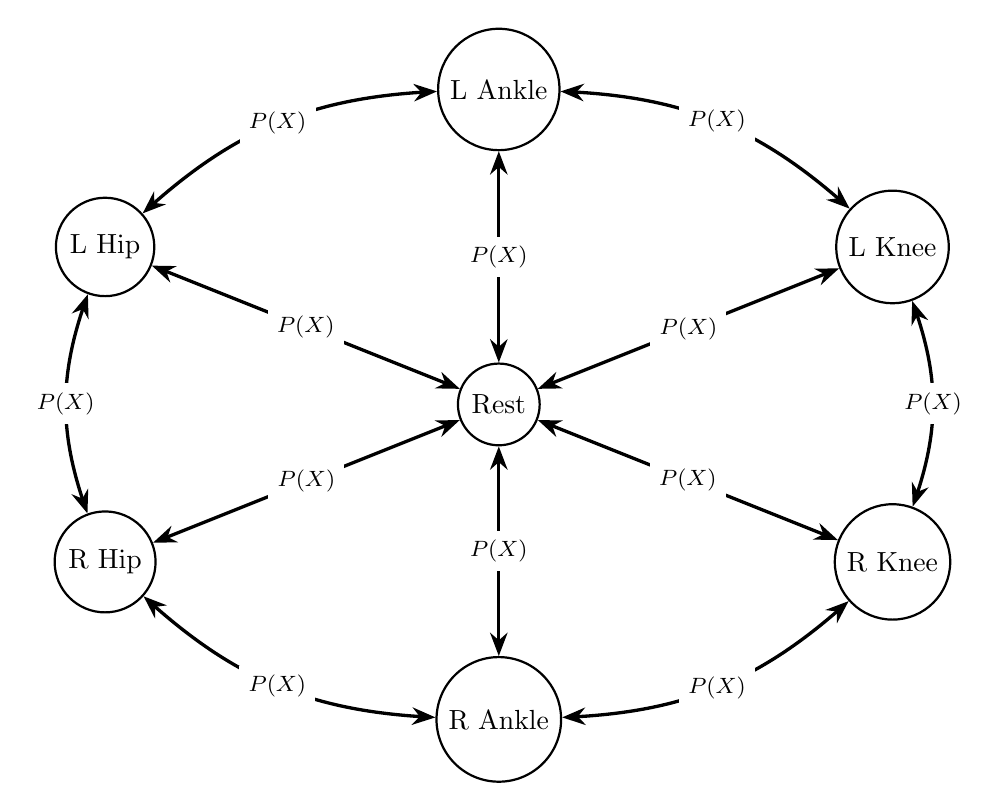
\begin{tikzpicture}
\begin{scope}[every node/.style={circle,thick,draw}]
    \node (Rest) at (0,0) {Rest};
    \node (LeftAnkle) at (0,4) {L Ankle};
    \node (LeftHip) at (-5,2) {L Hip};
    \node (LeftKnee) at (5,2) {L Knee};
    \node (RightAnkle) at (0,-4) {R Ankle};
    \node (RightHip) at (-5,-2) {R Hip};
    \node (RightKnee) at (5,-2) {R Knee};
    \end{scope}

\begin{scope}[>={Stealth[black]},
              every node/.style={fill=white,rectangle},
              every edge/.style={draw=black,very thick}]
    \path [<->] (Rest) edge node[pos=0.5] {\footnotesize{$P(X)$}} (LeftAnkle);
    \path [<->] (Rest) edge node[pos=0.5] {\footnotesize{$P(X)$}} (LeftKnee);
    \path [<->] (Rest) edge node[pos=0.5] {\footnotesize{$P(X)$}} (LeftHip);
    \path [<->] (Rest) edge node[pos=0.5] {\footnotesize{$P(X)$}} (RightHip);
    \path [<->] (Rest) edge node[pos=0.5] {\footnotesize{$P(X)$}} (RightKnee);
    \path [<->] (Rest) edge node[pos=0.5] {\footnotesize{$P(X)$}} (RightAnkle);
    \path [<->] (LeftHip) [bend left=20] edge node[pos=0.5] {\footnotesize{$P(X)$}} (LeftAnkle);
    \path [<->] (LeftHip) [bend right=20] edge node[pos=0.5] {\footnotesize{$P(X)$}} (RightHip);
    \path [<->] (RightHip) [bend right=20] edge node[pos=0.5] {\footnotesize{$P(X)$}} (RightAnkle);
    \path [<->] (RightAnkle) [bend right=20] edge node[pos=0.5] {\footnotesize{$P(X)$}} (RightKnee);
    \path [<->] (RightKnee) [bend right=20] edge node[pos=0.5] {\footnotesize{$P(X)$}} (LeftKnee);
    \path [<->] (LeftKnee) [bend right=20] edge node[pos=0.5] {\footnotesize{$P(X)$}} (LeftAnkle);
    \end{scope}

\end{tikzpicture}
\end{center}

Notably, they did not explicitly mention that one of the progressions could be from state to self state, but one can only assume this is true. So too, only seven states seems to limit the mobility of a patient.



\part[Project Proposal]{Project Proposal
            \vspace{0.2in}
            \begin{center}
            \begin{minipage}[l]{10cm}\small
                Man takes up the sword in order to shield the wound in his heart sustained in a far-off time beyond remembrance. Man wields the sword so that he may die smiling in some far-off time beyond perception. \newline
                -- Berserk by Kentaro Miura
            \end{minipage}
            \end{center}}

\chapter{Ramblings}

{\large \textcolor{red}{This section will largely be messy---likely for the coming years. It is for me to jot down ideas I have through reading.}}\newline

\begin{enumerate}
    \item Inhibit L-type VGCCs---likely need to use some kind of hydrogel with antagonists built in. 
    \item Optimize stiffness of paddles---or hydrogel, if we use the ACES system. 
    \item Optimize ECoG---that is, take up less space, maintain resolution, etc. to minimize invasiveness of surgery. 
\end{enumerate}

\subsubsection{Inhibit L-type VGCCs.}
It is well known by now that electrical stimulation combined with rehabilitation improves patient's ability to walk after SCI. 

\subsubsection{ACES Method.}

I like the ACES method as a starting point. It seems easy enough to implement, and can be built upon to arrive at some SCI method. Of course, I like that it is already integrated into a hydrogel setup. Some mild concerns are the 2 mA applied. It seems like quite a bit. 

\subsubsection{Biomaterials.}

The biomaterials possibilities are quite cool too. 

\subsubsection{Waveforms for Neuropathic Pain.}
Perhaps one can use a feedback mechanism, where the frequency of stimulation can be altered in order to dampen neural signals. You'd need to both read and write, essentially. Surely you can record brain waves responsible for feeling pain, and have a circuit edit itself to minimize them? $-->$ actually, dampening neural signals is a great example of a time to use the peak detection method, because you're only interested in magnitude. 

\vfill\pagebreak

\begin{center}
Thank you. There's one thing I'd like to leave you with: 
\end{center}

\vspace{2in}
            \begin{center}
            \begin{minipage}[l]{10cm}\small
            \textbf{The world is always full of the sound of waves.}\newline

            \textbf{The little fishes, abandoning themselves to the waves, dance and sing and play, but who knows the heart of the sea, a hundred feet down? Who knows its depth?}\newline
            \textbf{-- Musashi by Eiji Yoshikawa}
            \end{minipage}
            \end{center}
\vfill

\end{document}